%%%%%%%%%%%%%%%%%%%%%%%%%%%%%%%%%%%%%%%%%%%%%%%%%%%%%%%%%%%%%%%%%%%%%%%%%%%%%
%%                                                                           
%%  
%%									    
%%%%%%%%%%%%%%%%%%%%%%%%%%%%%%%%%%%%%%%%%%%%%%%%%%%%%%%%%%%%%%%%%%%%%%%%%%%%%
\documentclass[usenatbib]{mnras}

\usepackage{graphicx,fancyhdr,natbib,subfigure}
\usepackage{epsfig, epsf}
\usepackage{amsmath, cancel, amssymb}
\usepackage{lscape, longtable, caption}
\usepackage{multirow}
\usepackage{dcolumn}% Align table columns on decimal point
\usepackage{bm}% bold math
\usepackage{hyperref,ifthen}
\usepackage{verbatim}
\usepackage{color}
\usepackage[usenames,dvipsnames]{xcolor}
%% http://en.wikibooks.org/wiki/LaTeX/Colors



%%%%%%%%%%%%%%%%%%%%%%%%%%%%%%%%%%%%%%%%%%%
%       define Journal abbreviations      %
%%%%%%%%%%%%%%%%%%%%%%%%%%%%%%%%%%%%%%%%%%%
\def\nat{Nat} \def\apjl{ApJ~Lett.} \def\apj{ApJ}
\def\apjs{ApJS} \def\aj{AJ} \def\mnras{MNRAS}
\def\prd{Phys.~Rev.~D} \def\prl{Phys.~Rev.~Lett.}
\def\plb{Phys.~Lett.~B} \def\jhep{JHEP} \def\nar{NewAR}
\def\npbps{NUC.~Phys.~B~Proc.~Suppl.} \def\prep{Phys.~Rep.}
\def\pasp{PASP} \def\aap{Astron.~\&~Astrophys.} \def\araa{ARA\&A}
\def\pasa{PASA}
\def\jcap{\ref@jnl{J. Cosmology Astropart. Phys.}}%
\def\physrep{Phys.~Rep.}


\newcommand{\preep}[1]{{\tt #1} }

%%%%%%%%%%%%%%%%%%%%%%%%%%%%%%%%%%%%%%%%%%%%%%%%%%%%%
%              define symbols                       %
%%%%%%%%%%%%%%%%%%%%%%%%%%%%%%%%%%%%%%%%%%%%%%%%%%%%%
\def \Mpc {~{\rm Mpc} }
\def \Om {\Omega_0}
\def \Omb {\Omega_{\rm b}}
\def \Omcdm {\Omega_{\rm CDM}}
\def \Omlam {\Omega_{\Lambda}}
\def \Omm {\Omega_{\rm m}}
\def \ho {H_0}
\def \qo {q_0}
\def \lo {\lambda_0}
\def \kms {{\rm ~km~s}^{-1}}
\def \kmsmpc {{\rm ~km~s}^{-1}~{\rm Mpc}^{-1}}
\def \hmpc{~\;h^{-1}~{\rm Mpc}} 
\def \hkpc{\;h^{-1}{\rm kpc}} 
\def \hmpcb{h^{-1}{\rm Mpc}}
\def \dif {{\rm d}}
\def \mlim {m_{\rm l}}
\def \bj {b_{\rm J}}
\def \mb {M_{\rm b_{\rm J}}}
\def \mg {M_{\rm g}}
\def \qso {_{\rm QSO}}
\def \lrg {_{\rm LRG}}
\def \gal {_{\rm gal}}
\def \xibar {\bar{\xi}}
\def \xis{\xi(s)}
\def \xisp{\xi(\sigma, \pi)}
\def \Xisig{\Xi(\sigma)}
\def \xir{\xi(r)}
\def \max {_{\rm max}}
\def \gsim { \lower .75ex \hbox{$\sim$} \llap{\raise .27ex \hbox{$>$}} }
\def \lsim { \lower .75ex \hbox{$\sim$} \llap{\raise .27ex \hbox{$<$}} }
\def \deg {^{\circ}}
%\def \sqdeg {\rm deg^{-2}}
\def \deltac {\delta_{\rm c}}
\def \mmin {M_{\rm min}}
\def \mbh  {M_{\rm BH}}
\def \mdh  {M_{\rm DH}}
\def \msun {M_{\odot}}
\def \z {_{\rm z}}
\def \edd {_{\rm Edd}}
\def \lin {_{\rm lin}}
\def \nonlin {_{\rm non-lin}}
\def \wrms {\langle w_{\rm z}^2\rangle^{1/2}}
\def \dc {\delta_{\rm c}}
\def \wp {w_{p}(\sigma)}
\def \PwrSp {\mathcal{P}(k)}
\def \DelSq {$\Delta^{2}(k)$}
\def \WMAP {{\it WMAP \,}}
\def \cobe {{\it COBE }}
\def \COBE {{\it COBE \;}}
\def \HST  {{\it HST \,\,}}
\def \Spitzer  {{\it Spitzer \,}}
\def \ATLAS {VST-AA$\Omega$ {\it ATLAS} }
\def \BEST   {{\tt best} }
\def \TARGET {{\tt target} }
\def \TQSO   {{\tt TARGET\_QSO}}
\def \HIZ    {{\tt TARGET\_HIZ}}
\def \FIRST  {{\tt TARGET\_FIRST}}
\def \zc {z_{\rm c}}
\def \zcz {z_{\rm c,0}}

\newcommand{\ltsim}{\raisebox{-0.6ex}{$\,\stackrel
        {\raisebox{-.2ex}{$\textstyle <$}}{\sim}\,$}}
\newcommand{\gtsim}{\raisebox{-0.6ex}{$\,\stackrel
        {\raisebox{-.2ex}{$\textstyle >$}}{\sim}\,$}}
\newcommand{\simlt}{\raisebox{-0.6ex}{$\,\stackrel
        {\raisebox{-.2ex}{$\textstyle <$}}{\sim}\,$}}
\newcommand{\simgt}{\raisebox{-0.6ex}{$\,\stackrel
        {\raisebox{-.2ex}{$\textstyle >$}}{\sim}\,$}}

\newcommand{\Msun}{M_\odot}
\newcommand{\Lsun}{L_\odot}
\newcommand{\lsun}{L_\odot}
\newcommand{\Mdot}{\dot M}

\newcommand{\sqdeg}{deg$^{-2}$}
\newcommand{\hi}{H\,{\sc i}\ }
\newcommand{\lya}{Ly$\alpha$\ }
%\newcommand{\lya}{Ly\,$\alpha$\ }
\newcommand{\lyaf}{Ly\,$\alpha$\ forest}
%\newcommand{\eg}{e.g.~}
%\newcommand{\etal}{et~al.~}
\newcommand{\lyb}{Ly$\beta$\ }
\newcommand{\cii}{C\,{\sc ii}\ }
\newcommand{\ciii}{C\,{\sc iii}]\ }
\newcommand{\civ}{C\,{\sc iv}\ }
\newcommand{\SiII}{Si\,{\sc ii}\ }
\newcommand{\SiIV}{Si\,{\sc iv}\ }
\newcommand{\mgii}{Mg\,{\sc ii}\ }
\newcommand{\feii}{Fe\,{\sc ii}\ }
\newcommand{\feiii}{Fe\,{\sc iii}\ }
\newcommand{\caii}{Ca\,{\sc ii}\ }
\newcommand{\halpha}{H\,$\alpha$\ }
\newcommand{\hbeta}{H\,$\beta$\ }
\newcommand{\hgamma}{H\,$\gamma$\ }
\newcommand{\hdelta}{H\,$\delta$\ }
\newcommand{\oi}{[O\,{\sc i}]\ }
\newcommand{\oii}{[O\,{\sc ii}]\ }
\newcommand{\oiii}{[O\,{\sc iii}]\ }
\newcommand{\heii}{He\,{\sc ii}\ }
%\newcommand{\heii}{[He\,{\sc ii}]\ }
\newcommand{\nv}{N\,{\sc v}\ }
\newcommand{\nev}{Ne\,{\sc v}\ }
\newcommand{\neiii}{[Ne\,{\sc iii}]\ }
\newcommand{\alii}{Al\,{\sc ii}\ }
\newcommand{\aliii}{Al\,{\sc iii}\ }
\newcommand{\siiii}{Si\,{\sc iii}]\ }



\begin{document}

\title[Very high-$z$ Quasars]
        {Near and mid-infrared properties of known $z\geq5$ Quasars}
\author[Ross \& Cross]
       {Nicholas P. Ross$^{1}$\thanks{Corresponding Author: npross@roe.ac.uk} and Nicholas J. G. Cross$^{1}$
\\ 
$^1$Institute for Astronomy, University of Edinburgh, Royal Observatory, Edinburgh, EH9 3HJ, United Kingdom\\
}

\maketitle
\begin{abstract}
Lorem ipsum dolor sit amet, consectetur adipiscing elit. Aliquam porta
sodales est, vel cursus risus porta non. Vivamus vel pretium
velit. Sed fringilla suscipit felis, nec iaculis lacus convallis
ac. Fusce pellentesque condimentum dolor, quis vehicula tortor
hendrerit sed. Class aptent taciti sociosqu ad litora torquent per
conubia nostra, per inceptos himenaeos. Etiam interdum tristique diam
eu blandit. Donec in lacinia libero.
%%
Sed elit massa, eleifend non sodales a, commodo ut felis. Sed id
pretium felis. Vestibulum et turpis vitae quam aliquam convallis. Sed
id ligula eu nulla ultrices tempus. Phasellus mattis erat quis metus
dignissim malesuada. Nulla tincidunt quam volutpat nibh facilisis
euismod. Cras vel auctor neque. Nam quis diam risus.
\end{abstract}


\begin{keywords}
Astronomical data bases: surveys -- 
Quasars: general -- 
galaxies: evolution -- 
galaxies: infrared.
\end{keywords}


\section*{TO DOs}
{\bf For NPR: }
\begin{itemize}
\item Almost certainly want to compile M$_{\rm BH}$; hmmmm....
\item May well wanna try and get M$_{\star}$ too...!! (yuck); 
\item Filter curve plot with LSST, Euclid and even wide JWST filters...; 
\item Check with SpIES/SHELA (but only 3.4/4.6$\mu$m; 
\item Concentrate on NIR and W1/W2
\item SED dust plot with just W1/W2...
\item Check vs. Assef R90/C75 catalog.
\end{itemize}

\noindent
{\bf For NJGC: }
\begin{itemize}
\item Write the NIR data section(s) 
\end{itemize}

\noindent
{\bf For Both: }
\begin{itemize}
\item Need to decide what mags and mag system we are reporting, espeically in the 
NIR...
\item Depth/area QLF calculation to see whether the NIR surveys have been fully mined...
\end{itemize}


%%%%%%%%%%%%%%%%%%%%%%%%%%%%%%%%%%%%%%%%%%%%%%%%%%%%%%%%%%%%%%%%%%
%%%%%%%%%%%%%%%%%%%%%%%%%%%%%%%%%%%%%%%%%%%%%%%%%%%%%%%%%%%%%%%%%%
%%
%%  S E C T I O  N   1         S E C T I O  N   1           S E C T I O  N   1       S E C T I O  N   1
%%  S E C T I O  N   1         S E C T I O  N   1           S E C T I O  N   1       S E C T I O  N   1
%%  S E C T I O  N   1         S E C T I O  N   1           S E C T I O  N   1       S E C T I O  N   1
%%
%%%%%%%%%%%%%%%%%%%%%%%%%%%%%%%%%%%%%%%%%%%%%%%%%%%%%%%%%%%%%%%%%%
%%%%%%%%%%%%%%%%%%%%%%%%%%%%%%%%%%%%%%%%%%%%%%%%%%%%%%%%%%%%%%%%%%
\section{Introduction}
Very high redshift quasars (VH$z$Q; and defined here to have redshifts
$z\geq5.00$) are excellent probes of the early Universe. This includes
studies of the Epoch of Reionization for hydrogen \citep[see e.g.][for
reviews]{Fan2006review, Mortlock2016}, the formation and build-up of
supermassive black holes \citep[e.g., ][]{Rees1984, WyitheLoeb2003,
Volonteri2010, Agarwal2016, Valiante2018, Latif2018} and early metal
enrichment \citep[see e.g., ][]{Simcoe2012, Chen2017, Bosman2017}.

The build-up of SMBHs via accretion is important due to the desire to
understand the evolution of the black hole mass function (BHMF) and
since there is a remarkable similarity between cosmic star-formation
rate density (SFRD) and black hole accretion rate (BHAR). The SFRD and
BHAR trace each other \citep[with a normalisation factor of
$\sim3000$,][]{Willott2013b, MadauDickinson2014} across redshifts
$z=0-4$.  However, new results \citep[e.g., ][]{Vito2018a, Calhau2018}
suggest that the SFRD and BHAR do {\it not} have the same evolutionary form
at higher redshift, $z>4$. The physical reasons for this are currently very poorly
understood.  For the high-$z$ QSOs that we can measure BHAR and SFR, most
have BHAR $\gg 10^{-3}$ SFR, indeed {\it Herschel}-detected sources at
$z\simeq.8$ have $L_{\rm SF} \simeq L_{\rm AGN}$ \citep[e.g.,
][]{Netzer2014} and {\it Herschel}-detected quasars show no evolution
in the $M_{\rm BH} - M_{\star}$ relation from $z\sim2$ to $z\sim0$.
where $M_{\rm BH}, M_{\rm bulge}, M_{\star}$ are the SMBH mass,
stellar mass of the bulge and galaxy total stellar mass,
respectively. The evolution and potential importance of the SFRD and BHAR 
link is a key outstanding problem in contemporary astrophysics, 
potentially explaining the galaxy-black hole scaling relations. 
However, there may also simply be a non-causal origin of the black-hole 
galaxy scaling relations \citep{Jahnke2011}.

Quasars are also known to be prodigious emitters of infrared emission,
thought to be from the thermal emission of dust grains heated by
continuum emission from the accretion disc \citep[][]{Hill2014,
Hickox2017}.  Observations in the mid-infrared, e.g. $\sim$3-30$\mu$m
allow discrimination between AGN\footnote{Historically, ``quasars'' and
``Active Galactic Nuclei (AGN)'' have described different
luminosity/classes of objects, but here we use these terms
interchangeably (with a preference for quasar) in recognition of the
fact that they both describe accreting supermassive black holes
\citep[e.g.][]{Haardt2016book}.}  and passive galaxies due to the
1.6$\mu$m ``bump'' entering the MIR at $z\approx0.8-0.9$ \citep[e.g.,
][]{Wright1994, Sawicki2002, Lacy2004, Stern2005, Richards2006b,
Timlin2016} as well as AGN and star-forming galaxies due to the
presence of Polycyclic Aromatic Hydrocarbon (PAHs) at $\lambda >3\mu$m
\citep[e.g., ][]{Yan2007, Tielens2008}.

\citet{Jiang2006dust} and \citet{Jiang2010} report on the discovery of
a quasar without hot-dust emission in a sample of 21 $z\approx6$
quasars. Such apparently hot-dust-free quasars have no counterparts at
low redshift. Moreover, those authors demonstrate that the hot-dust
abundance in the 21 quasars builds up in tandem with the growth of the
central black hole.

WISE mapped the sky in 4 passbands, in bands centered at wavelengths
of 3.4, 4.6, 12, and 23$\mu$m.  In total the release all sky
``ALLWISE'' catalog, contains nearly 750 million detections at
high-significance\footnote{\href{wise2.ipac.caltech.edu/docs/release/allwise/expsup/sec2\_1.html}{wise2.ipac.caltech.edu/docs/release/allwise/expsup/sec2\_1.html}}. \citet{Assef2013},
\citet{Stern2012}. \citet{Blain2013} presented WISE mid-infrared (MIR)
detections of 17 (55\%) of the then known 31 quasars at $z >
6$. However, \citet{Blain2013} was compiled with the WISE `All-Sky'
data release, as opposed to the superior ``AllWISE'' catalogs. That
sample only examined the 31 known $z>6$ quasars; our sample has 148
objects with redshift $z \geq 6.00$.

Here we update \citet{Jiang2010} and \citet{Blain2013} \citep[along
with Table 8 of][]{Banados2016}. Our motivations are numerous and
include: {\it (i)} establishing the first complete catalogue of
$z>5.00$ quasars since the pioneering work from SDSS; {\it (ii)}
reporting homogenous near-infrared photometry for the quasars; {\it
(iii)} making the first study of NIR variability of the VHzQ
population and {\it (iv)} establishing the photometric properties for
upcoming surveys and telescopes, e.g. the Large Synoptic Survey
Telescope (LSST) \footnote{\href{https://www.lsst.org}{{lsst.org}}},
ESA {\it
Euclid}\footnote{\href{https://sci.esa.int/euclid/}{sci.esa.int/euclid/}}
and the {\it James Webb Space Telescope}
(JWST)\footnote{\href{https://www.jwst.nasa.gov/}{jwst.nasa.gov};
\href{https://sci.esa.int/jwst/}{sci.esa.int/jwst};
\href{https://www.asc-csa.gc.ca/eng/satellites/jwst/}{www.asc-csa.gc.ca/eng/satellites/jwst};
\href{https://jwst.stsci.edu/}{jwst.stsci.edu}}

We chose redshift $z=5.00$ as our lower redshift limit due to a combination 
of garnishing a large sample, adequately spanning physical properties 
(e.g. luminosity, age of the Universe) and to incorporate what knowledge 
we've gained over the last couple of decades since $z>5$ quasars were 
discovered. 

This paper can be considered an update of \citet{Blain2013} and also
an extension of parts of \citet{Banados2016}, with the latter study reporting
WISE W1, W2, W3 and W4 magnitudes for Panoramic Survey Telescope and Rapid Response System 1 
\citep[Pan-STARRS1, PS1;][]{Kaiser2002, Kaiser2010}, but with no  
further investigation into the reddest WISE waveband for the VH$z$Qs.
%%
\citet{Banados2016} reports and investigates the W1, W2 and W3 properties
of quasars at $z > 5.6$.

Because of established conventions, we report SDSS $ugriz$ magnitudes on the AB zero-point system \citep{Oke_Gunn1983, Fukugita1996}, while the WISE W1 − 4 magnitudes are calibrated on the Vega system (Wright et al. 2010). For WISE bands, $m_{\rm AB} = m_{\rm Vega} + m$ where m = (2.699, 3.339, 5.174, 6.66) for W1, W2, W3 and W4, respectively \citep{Cutri2011, Brown2014b}. \citet{Brown2014b}, in PASA, is the paper about Recalibrating the Wide-field Infrared Survey Explorer (WISE) W4 Filter. We make use of the Explanatory Supplement to the WISE All-Sky Data Release, as well as the WISE AllWISE Data Release  Products online. 
All optical ($ugriz$ bands) magnitudes are given in the AB system. 
{\bf Need to decided 
All near-infrared  ($y/YJHK$) are also given in the AB system.  

We use a flat $\Lambda$CDM cosmology with $H0 = 67.7$ km s$-1$ Mpc$−1$,  $\Omega_{\rm M} = 0.307$, and $\Omega_{\Lambda} = 0.693$ (Planck Collaboration et al. 2016) in order to be consistent with \citet{Banados2016}. 


%%%%%%%%%%%%%%%%%%%%%%%%%%%%%%%%%%%%%%%%%%%%%%%%%%%%%%%%%%%%%%%%%%
%%%%%%%%%%%%%%%%%%%%%%%%%%%%%%%%%%%%%%%%%%%%%%%%%%%%%%%%%%%%%%%%%%
%%
%%  S E C T I O  N   2         S E C T I O  N   2           S E C T I O  N   2       S E C T I O  N   2
%%  S E C T I O  N   2         S E C T I O  N   2           S E C T I O  N   2       S E C T I O  N   2
%%  S E C T I O  N   2         S E C T I O  N   2           S E C T I O  N   2       S E C T I O  N   2
%%
%%%%%%%%%%%%%%%%%%%%%%%%%%%%%%%%%%%%%%%%%%%%%%%%%%%%%%%%%%%%%%%%%%
%%%%%%%%%%%%%%%%%%%%%%%%%%%%%%%%%%%%%%%%%%%%%%%%%%%%%%%%%%%%%%%%%%
\section{Data}
\begin{figure*}
%%trim=l b r t
  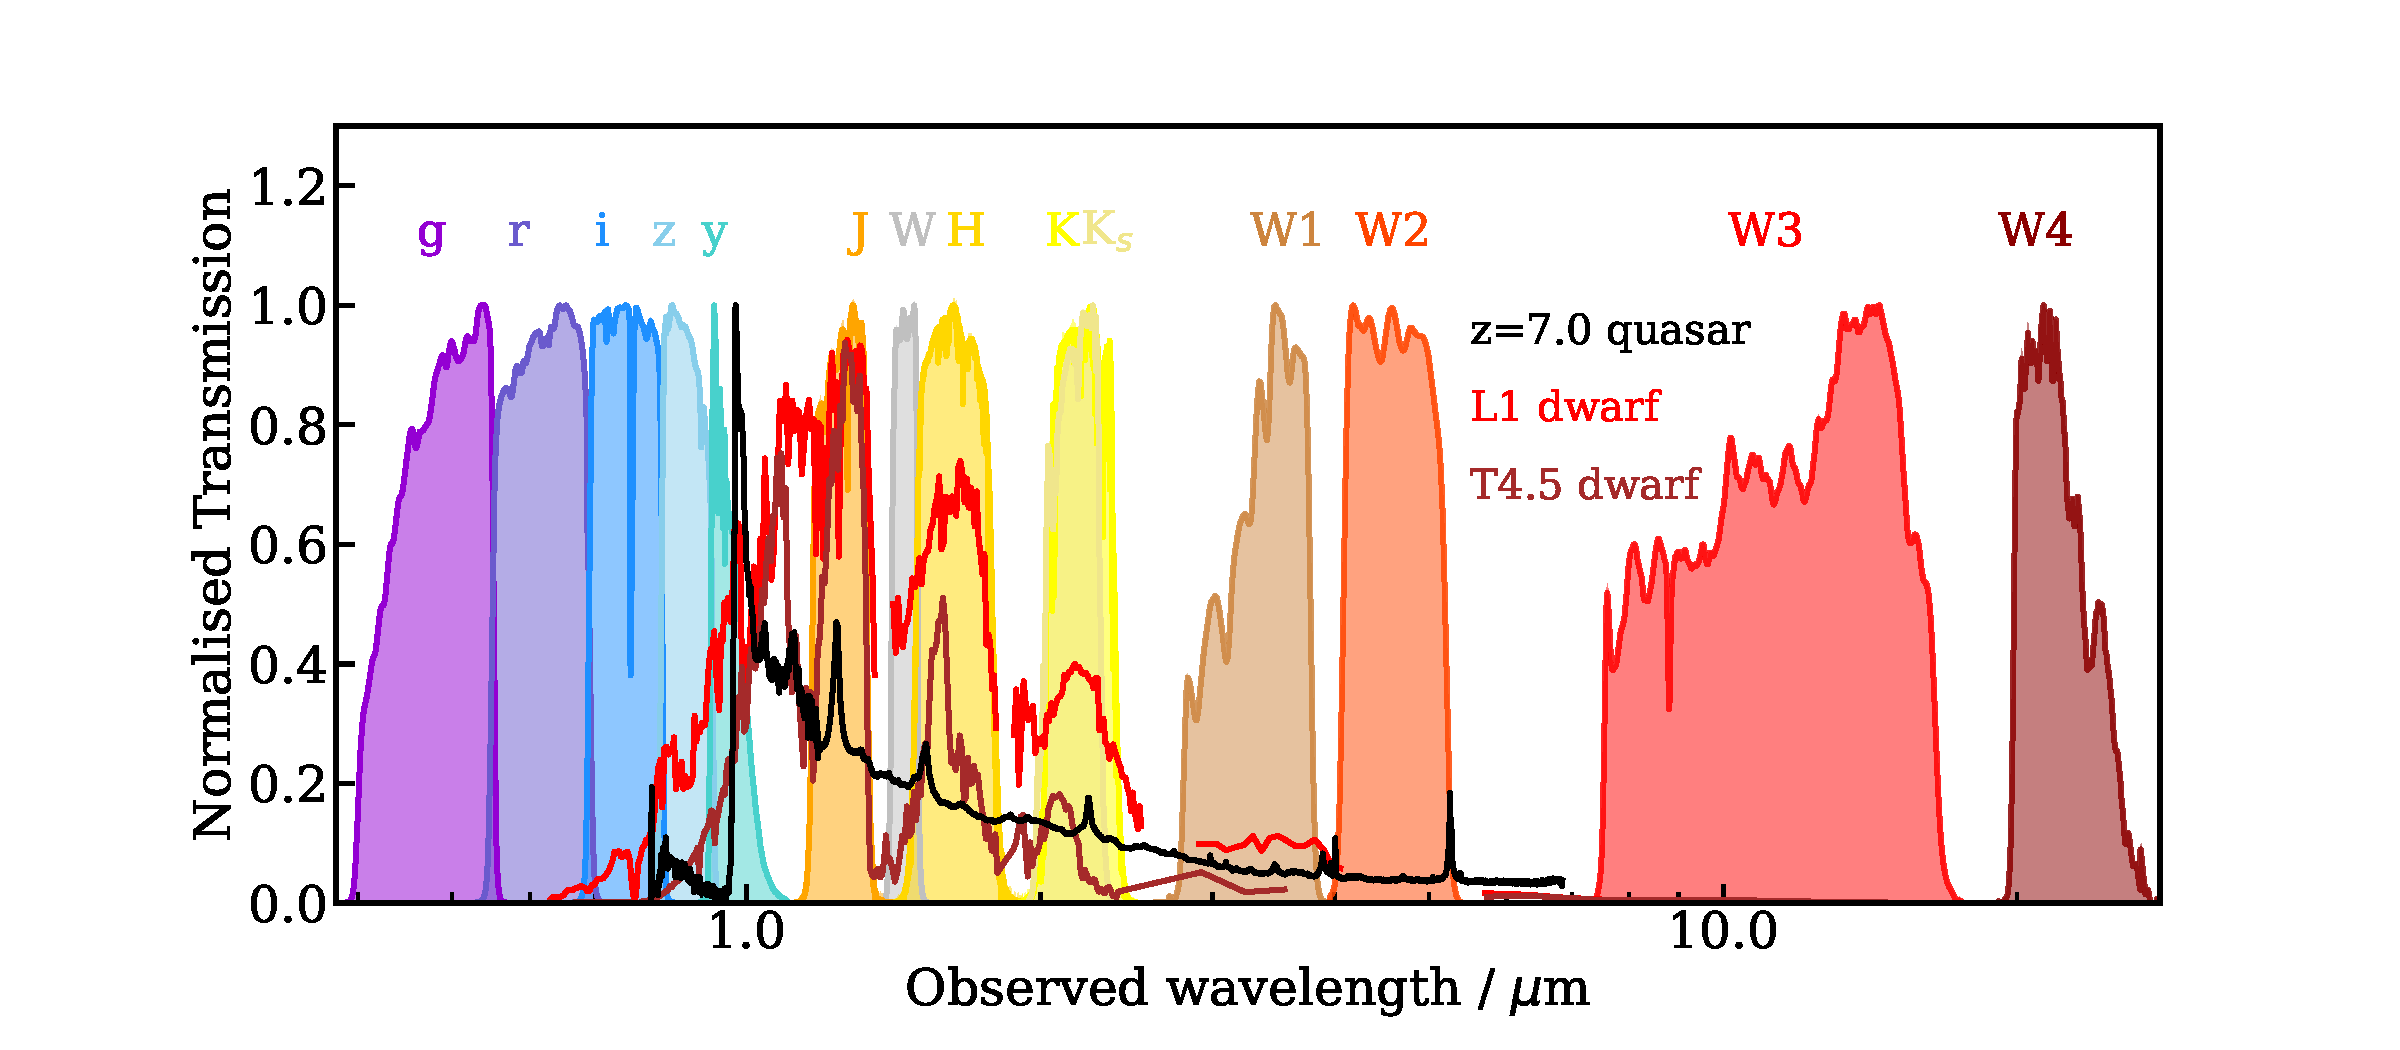
\includegraphics[width=18.6cm, clip,trim=14mm 4mm 10mm 10mm]
  {/cos_pc19a_npr/programs/quasars/highest_z/SEDs/filters_vs_QSOstars_20180704.pdf}
  \centering
  \caption[]
  {The spectral bands used by different survey telescopes and that are relevant here.}
  \label{fig:filters}
\end{figure*}

\pagestyle{empty}
\begin{landscape}
%\onecolumn
 % \begin{landscape}
%\small  %\footnotesize \scriptsize \tiny
\begin{table}
\begin{center}
\begin{tabular}
%{|l|l|l|l|r|r|r|r|r|r|r|r|r|r|r|r|r|r|r|r|r|r|r|r|l|}
%{ l l l l r r r r r r r r r r r r r r r r r r r r l }
{ l l l l l l l l l l l l l l l l l l l l l l l l l }
\hline \hline
  \multicolumn{1}{ c }{na} &
  \multicolumn{1}{c }{desig} &
  \multicolumn{1}{c }{ra\_hms} &
  \multicolumn{1}{c }{dec\_dms} &
  \multicolumn{1}{c }{ra} &
  \multicolumn{1}{c }{dec} &
  \multicolumn{1}{c }{redshift} &
  \multicolumn{1}{c }{mag} &
  \multicolumn{1}{c }{M1450} &
  \multicolumn{1}{c }{errM1450} &
  \multicolumn{1}{c }{ra\_WISE} &
  \multicolumn{1}{c }{dec\_WISE} &
  \multicolumn{1}{c }{w1mag} &
  \multicolumn{1}{c }{w1err} &
  \multicolumn{1}{c }{w1snr} &
  \multicolumn{1}{c }{w2mag} &
  \multicolumn{1}{c }{w2err} &
  \multicolumn{1}{c }{w2snr} &
  \multicolumn{1}{c }{w3mag} &
  \multicolumn{1}{c }{w3err} &
  \multicolumn{1}{c }{w3snr} &
  \multicolumn{1}{c }{w4mag} &
  \multicolumn{1}{c }{w4err} &
  \multicolumn{1}{c }{w4snr} &
  \multicolumn{1}{c }{ref} \\
\hline
  PSO & J000.3401+26.8358 & 00:01:21.63 & +26:50:09.17 & 0.34011348 & 26.83588138 & 5.75 & 19.52 & -27.16       & 9.99 & 0.3400887 & 26.835823        &     16.373 & 0.066 & 16.5 & 15.266 & 0.107 & 10.2 & 12.594 & 0.492 & 2.2 & 8.756 & -9.99 & 1.1 & 1/1/1\\
  SDSS & J0002+2550 & 00:02:39.39 & +25:50:34.80 & 0.66411726 & 25.84304425 & 5.82 & 19.39 & -27.31                 & 9.99 & 0.6641312 & 25.8430852      & 16.162 & 0.057 & 19.0 & 15.542 & 0.127 & 8.5 & 12.416 & 0.423 & 2.6 & 8.683 & -9.99 & 1.2 & 5/22/1\\
  SDSS & J0005-0006 & 00:05:52.34 & -00:06:55.80 & 1.4680833 & -0.1154999 & 5.85 & 20.98 & -25.73                       & 9.99 & 1.4683933 & -0.1154292     & 17.299 & 0.16 & 6.8 & 17.043 & -9.99 & 0.2 & 12.445 & -9.99 & -1.1 & 9.008 & -9.99 & -0.3 & 5/12/1\\
  PSO & J002.1073-06.4345 & 00:08:25.77 & -06:26:04.60 & 2.10739 & -6.43456 & 5.93 & 20.41 & -26.32                    & 9.99 & 2.1073696 & -6.4345725      & 16.809 & 0.107 & 10.1 & 15.684 & 0.141 & 7.7 & 11.892 & -9.99 & 1.5 & 8.759 & -9.99 & 0.2 & 1;43/1/1\\
  SDWISE & J0008+3616 & 00:08:51.43 & +36:16:13.49 & 2.2142917 & 36.2704138 & 5.17 & 19.12 & -27.34                 & 9.99 & 2.2142355 & 36.2704366       & 16.045 & 0.052 & 20.7 & 15.373 & 0.092 & 11.8 & 12.043 & -9.99 & 1.8 & 8.786 & -9.99 & 1.1 & Wang2016\\
  PSO & J002.3786+32.8702 & 00:09:30.89 & +32:52:12.94 & 2.37870183 & 32.87026179 & 6.1 & 21.13 & -25.65        & 9.99 & 2.3787018 & 32.8702618       & -99.99 & -9.99 & -9.9 & -99.99 & -9.99 & -9.9 & -99.99 & -9.99 & -9.9 & -9.99 & -9.99 & -9.9 & 1/1/1\\
  SDSS & J0017-1000 & 00:17:14.68 & -10:00:55.4 & 4.3111666 & -10.01539722 & 5.011 & 99.99 & -99.99                 & 9.99 & 4.3111476 & -10.0154269      & 15.936 & 0.055 & 19.7 & 15.167 & 0.094 & 11.5 & 12.026 & 0.334 & 3.2 & 8.52 & -9.99 & 1.2 & DR7\_W16\\
  PSO & J004.3936+17.0862 & 00:17:34.47 & +17:05:10.70 & 4.39361347 & 17.08630447 & 5.8 & 20.69 & -26.01        & 9.99 & 4.3936134 & 17.0863047        & -99.99 & -9.99 & -9.9 & -99.99 & -9.99 & -9.9 & -99.99 & -9.99 & -9.9 & -9.99 & -9.99 & -9.9 & 1/1/1\\
  PSO & J004.8140-24.2991 & 00:19:15.38 & -24:17:56.98 & 4.81408 & -24.29916 & 5.68 & 19.43 & -27.24                 & 9.99 & 4.814116 & -24.2990993        &   16.281 & 0.069 & 15.8 & 15.569 & 0.116 & 9.4 & 12.123 & 0.344 & 3.2 & 8.82 & -9.99 & 0.5 & 1/1/1\\
  VDES & J0020-3653 & 00:20:31.46 & -36:53:41.8 & 5.1311237 & -36.8949476 & 6.9 & 99.99 & -99.99                        & 9.99 & 5.1311237 & -36.8949476     & 16.844 & 0.094 & 11.6 & 16.354 & 0.204 & 5.3 & 12.679 & -9.99 & -0.1 & 8.342 & -9.99 & 0.8 & DES-VHS\_inprep\\
\hline \hline
\end{tabular}
\caption{All 425 $z\geq5.00$ quasars that have been spectroscopically confirmed as of 2018 June. 
  The first ten objects are given here as guidance to the format of the data table. The full table  can be found online.} 
\label{tab:THE_TABLE}
  \end{center}
\end{table}
\normalsize 
  \end{landscape}
\twocolumn
\pagestyle{plain}


Table~\ref{tab:THE_TABLE} gives the salient details for the objects
used in this study. We use all the $z\geq5.00$ quasars that
have been discovered and spectroscopically confirmed as of the time of
writing (2018 June). We report near-infrared ($yYJHK$-bands)
and mid-infrared (WISE W1/2/3/4) photometry and give our caculcated 
$M_{1450}$

\begin{table}
\begin{tabular}{l r l}
\hline  \hline
Survey   & \# VH$z$Qs & Notes  \\
\hline  
  ATLAS      &    4    &  \\
  CFHQS     &  20    &  \\
  DELS        &    2    &  \\
  ELAIS       &    1    &  \\
  FIRST       &    1    &  \\
  HSC         &    8    &  \\
  IMS          &   1     &  \\
  MMT        &  12    &  \\
  NDWFS    &  1      &  \\
  PSO          &    84  & \\
  RD           &  1       & \\
  SDSS        & 156       & \\
  SOUV       & 20       & \\
  SDWISE    & 27& \\
  SHELLQs  & 55 & \\
  ULAS       & 10& \\
  VDES       & 11& \\
  VIK          & 9 &\\
  VIMOS     & 1& \\
\hline  \hline
\end{tabular}
\caption{ATLAS \citet{Shanks2015}; }
      \label{tab:surveys}
\end{table}



\subsection{Very high redshift quasars}
In Table~\ref{tab:THE_TABLE} we give the discovery reference for the
VH$z$Qs noting that some objects were discovered independently and
contemporaneously.  The redshifts for the VH$z$Qs generally come from
the measurement of broad UV/optical emission lines. Where 
there are far infra-red emission lines e.g. \cii~158 micron, we report 
these, but at the level of our current analysis broadline redshifts are
sufficient. 

Specifically, we use data from: \citet{Fan2000}, \citet{Fan2001c},
\citet{Fan2003} , \citet{Fan2004}, \citet{Mahabal2005},
\citet{Cool2006}, \citet{Fan2006}, \citet{Goto2006},
\citet{McGreer2006}, \citet{Carilli2007}, \citet{Kurk2007},
\citet{Stern2007}, \citet{Venemans2007}, \citet{Willott2007},
\citet{Jiang2008}, \citet{Wang2008}, \citet{Jiang2009}, \citet{Kurk2009}, 
\citet{Mortlock2009}, \citet{Willott2009}, \citet{Carilli2010}, 
\citet{Wang2010}, \citet{Willott2010a}, \citet{Willott2010b}, 
\citet{DeRosa2011}, \citet{Mortlock2011}, \citet{Wang2011}, 
\citet{Zeimann2011}, \citet{Morganson2012}, \citet{Venemans2012}, 
\citet{McGreer2013}, \citet{Venemans2013}, \citet{Wang2013}, 
\citet{Willott2013b}, \citet{Banados2014}, \citet{Calura2014}, 
\citet{Leipski2014}, \citet{Banados2015a}, \citet{Banados2015b}, 
\citet{Becker2015}, \citet{Carnall2015}, \citet{Jiang2015}, 
\citet{Kashikawa2015}, \citet{Kim2015}, \citet{Reed2015}, 
\citet{Venemans2015a}, \citet{Venemans2015b}, \citet{Willott2015}, 
\citet{Wu2015}, \citet{Venemans2016}, \citet{Wang2016_WISE}, 
\citet{Matsuoka2016}, \citet{WangR2016}, \citet{Mortlock2011},
\citet{McGreer2013}, \citet{Venemans2013}, \citet{Venemans2013},
\citet{Venemans2015a}, \citet{Venemans2015b}, \citet{Banados2016},
\citet{Matsuoka2016}, \citet{Reed2017}, \citet{Wang2017},
\citet{Mazzucchelli2017}, \citet{Ikeda2017}, \citet{Tang2017},
\citet{Koptelova2017}, \citet{Banados2018}, \citet{Matsuoka2018a} 
and \citet{Matsuoka2018b}. 
        
\subsection{Optical Photometry}
\subsubsection{Pan-STARRS1 (PS1)} 
We query the Panoramic Survey Telescope and Rapid Response System
(Pan-STARRS)\footnote{\href{https://outerspace.stsci.edu/display/PANSTARRS}{https://outerspace.stsci.edu/display/PANSTARRS}}
Data Release 1 (DR1) Catalog Archive Server Jobs System (CasJobs)
service at
\href{http://mastweb.stsci.edu/ps1casjobs/}{mastweb.stsci.edu/ps1casjobs/}.
The PS1 survey observed the 30,000 deg$^{2}$ of sky north of
declination $-30$ degrees in five filters $grizy$.  Pan-STARRS1 (PS1)
is the first part of Pan-STARRS to be completed and is the basis for
the DR1.  \citet{Chambers2016}, \citet{Magnier2016a},
\citet{Waters2016}, \citet{Magnier2016b}, \citet{Magnier2016c} and
\citet{Flewelling2016} describe the instrument, survey, and data
analyses.  The principal science product of the PS1 survey is the
catalog accessible through the CasJobs interface.

We query and return the mean PSF magnitudes from the $grizy$ filters
({\tt MeanPSFMag}) which are in the AB system for our 425 VH$z$Q
sample. Details of our SQL and links to the main tables are given
in~\ref{sec:PS1_SQL}.


%\newpage
\subsection{Near-infrared photometry}
Due to their selection of being very faint/undetected in the
observed-frame optical but bright in the observed frame near-infrared,
VH$z$Qs are generally detected in the near-infrared $yYJHK$-bands
\citep[$\approx$0.98-2.38$\mu$m; e.g., ][]{Peth2011}.

We query the WFCAM Science Archive
\citep[\href{http://wsa.roe.ac.uk/}{WSA}; ][]{Hambly2008} which
reports NIR photometry from the Wide Field Camera \citep[WFCAM;
][]{Casali2007} on the United Kingdom Infrared Telescope (UKIRT).
Data from the VIRCAM (VISTA InfraRed CAMera) on the VISTA
\citep[Visible and Infrared Survey Telescope for Astronomy;
][]{Emerson2006, Dalton2006} is also given in the WSA.

Quasars are known to vary (both photometrically and spectroscopically)
and very high-$z$ quasars under going super-Eddington accretion during
a rapid BH growth phase are prime candidates for this variation.
Therefore, with repeat observations over many epochs availble via the
WSA, we have a choice to make for how we report the photometry. After
tests, we decide to give the NIR photometry averaged on 4 week
observed timescales. This time bracket is chosen as a good compromise
between maximising signal-to-noise while keeping the cadence high. At
our observed redshifts, we sample $\lesssim1$week in the rest-frame
and luminous quasars are not expected to vary on timescales quicker
than this \citep[e.g., ][]{Lawrence2016_ASPC}. 
 
We give our recipe and SQL query syntax in Appendix~\ref{sec:SQL}.


\section{NIR Data}

The near-infrared data in this paper comes from the Wide Field Astronomy Unit's
(WFAU) Science Archives for UKIRT-WFCAM, the WFCAM Science Archive
\citep[WSA][]{WSA} and VISTA-VIRCAM, the VISTA Science Archive
\citep[VSA][]{VSA}. These archives were developed for the VISTA Data Flow System
\citep[VDFS][]{VDFS}.

In this paper we include all non-proprietary WFCAM data, which covers all
public surveys and PI projects from Semester 05A to 1st January 2017 and all
non-proprietary VISTA data, which covers all public surveys and PI projects from
science verification (200910..) to 1st April 2016, to get as much coverage as
possible. Hence, the NIR is extremely heterogeneous. 

The data was processed using a forced photometry, or matched-aperture
photometry. A pipeline for this has been developed by WFAU, but
has not yet been incorporated into the main VDFS pipeline. Full details of the
matched-aperture pipeline (MAP) will appear in a forthcoming paper, Cross et al.
2018, in prep, and has also been discussed in \citet{Cross2013} and \citet{Cross2017}.
We will give the pertinent points of the MAP and specific details of these data sets below.


\subsection{Selection of NIR}

The first step of the process was to ingest the catalogue of VHzQs into
the WSA/VSA. These data are in the table \verb+finalQsoCatalogue+. Next we set
up new programmes WSERV1000, VSERV1000 in the WSA and VSA respectively. We
assign all frames that contain the high-z QSO based on WCS information in the
WSA to WSERV1000, but adding a new line to the table \verb+ProgrammeFrame+ and
same in VSA for VSERV1000. Assigning these frames to a separate programme allows
us to process them together and put them into a single release. 

\subsection{Setup Matched Aperture Product}

Add a new entry \verb+RequiredMatchedApertureProduct+

\begin{itemize}
\item mapID	archiveName	programmeID	extractor	mapType	name	description	selection	finalProductTable	addSurveyList
\item 1	1	WSA	10999	CASU	2	highzQsoMap	Variability via matched apertures for set of high-z QSOs	SELECTSTR qsoID,ra,dec FROMSTR finalQsoCatalogue	highzQsoMapVariability	NONE
\end{itemize}

Explain

Entries in \verb+RequiredMapAverages+

Add table?
\begin{table*}
  \begin{center}
    \setlength{\tabcolsep}{4pt}
    \begin{tabular}{lll lll lll l}
\hline \hline
                &  programmeID &	mapID &	setupID  &	description               &	useDeeps  &	useHighProd &	timeScale	    &  nEpochs     &	overLaps\\
\hline
      1	& 10999	           &    1       &	1            &      Average over a week	 &     0        & 	NONE            &	+7.000000  &	-99999999 &	0\\
      2	& 10999             & 	 1	  & 2   	     & Average over a fortnight &	0        &	NONE	&+14.000000	&-99999999 &	0\\
      3	& 10999	           &    1  	 & 3	             & Average over a month	&      0        &	NONE	&+30.000000	&-99999999 &	0\\
      4	& 10999             & 	 1	 & 4	              & Average over 10 epochs &	0        &	NONE	&-9.999995E008 &	10 &	0\\
      5	& 10999             &	 1	 & 5	             & Average over 6 months   &	0        &	NONE	&+183.000000 &	-99999999 &	0\\
      6	& 10999            &	 1	 & 6	           & Average over whole time  &	0        &	NONE	&-1.000000 &	-99999999 &	0\\
      \hline \hline
      \label{tab:The_Numbers}
    \end{tabular}
    \caption{}
  \end{center}
\end{table*}


Explain
 
\subsection{Processing MAP data}

A set of apertureIDs were created in \verb+MapApertureIDshighzQsoMap+, based on
the \verb+RequiredMatchedApertureProduct+ {\bf selection} value. This may
seem unnecessary layer since it is a one-to-one match with \verb+finalQsoCatalogue+,
but the layer is a general abstraction that allows multiple sources of
catalogue, and multiple types\ldots
Entries added to \verb+MapSurveyTables+ $\Rightarrow$ not pertinent

\subsubsection{Forced photometry}
CASU's \verb+imcore_list+ was run on each frame assigned to the programme with
the input list equal to objects selected to be within \ldots of the multiframe
centre. In this case, where there are 424 QSOs spread across the sky, there is
typically 1 object per multiframe, but many have two and one,
multiframeID=2614475 in the VSA, has 3 objects. The output of \verb+imcore_list+
is a multi-extension FITS binary table, with identical columns to the CASU FITS
binary tables produced using the CASU \verb+imcore+, the basis of all WFCAM and
VISTA survey products and also familiar to many astronomers through the INTWFS
\citep{}, and VST-ATLAS and -VPHAS \citep{}. Since forced photometry can be run
in many ways on a particular image, a single science frame is not
necessarily linked to a single MAP catalogue, so the \verb+MapFrameStatus+ table
links images ({\bf multiframeID}) to catalogues ({\bf catalogueID}) and gives
information on what processing stage they are at ({\bf bitProcessingFlag}),
whether they have been ingested ({\bf isIngested}), or what quality control has
been run on them ({\bf ppErrBitsStatus}).

For matched aperture measurements, we process these binary tables using the same
software, as the standard extracted catalogues, but implement a few different
processes. We calculate both Luptitudes \citep{Luptitudes}, and calibrated fluxes,
see Eqn~\ref{eq:jky}. 


\begin{equation}
F^{calib} = f\times10^{-0.4*(ZP+VAB-8.90+corr)} 
\label{eq:jky}
\end{equation}

\noindent where $f$ is the measured flux in ADU, $ZP$ is the zeropoint of
frame, $VAB$ is the Vega-to-AB correction for the filter, and $corr$ are the
various correction terms, e.g. distortion correction, scattered light
correction, aperture correction, see \citep{Hambly2008, Cross2012}. 

Once all data is processed, the data are ingested into
\verb+wserv1000MapRemeasurement+ and \verb+vserv1000MapRemeasurement+
respectively. These tables are similar in structure to \verb+lasDetection+
described in \citep{Hambly2008} or other UKIDSS or VISTA detection tables. One of
the main differences is the primary key which is ({\bf apertureID},{\bf
catalogueID}) rather than ({\bf multiframeID},{\bf extNum},{\bf seqNum}),
reflecting the fact that these are forced photometry on a known set of apertures
and a set of catalogues, rather than detections above a threshold in a set of
detector extensions to image multiframes.

\subsubsection{Averaging matched photometry}

Unfortunately the photometry in a single epoch image often has low
signal-to-noise. The advantage of matched aperture photometry on QSOs is that
co-adding is relatively simple: if each epoch is taken in the same aperture
(assuming the astrometry is correct) and the aperture photometry has been
corrected to total: the standard aperture corrections work well for point
sources then averaging the calibrated photometry should give as good as
extracting from a deep stack. In fact it will almost certainly do better, since
the images in some cases are taken from multiple projects with different
pointings. In addition, corrections such as scattered light, pixel distortion
and aperture corrections will be more complex, if not impossible to apply to
deep-stacks but will be automatically applied in the averaging of forced
photometry. 

We average the aperture corrected calibrated fluxes (e.g. {\bf aperJky3}), and
then convert to magnitudes or luptitudes. Since we do not have a deep image for
each set of averages, we cannot calculate non-aperture corrected values, so the
photometry is only appropriate for point-sources. 

\begin{equation}
\bar{F} = \frac{\sum_i^N (w_i\,F_i)}{\sum_i^N w_i}  
\label{eq:avg}
\end{equation}

\noindent where $F_i$ is the $i^{th}$ epoch measurement of a parameter to be
averaged such as the aperture corrected calibrated flux in a $1\arcsec$ aperture
({\bf aperJky3}) and $\bar{F}$ is the weighted mean average of this parameter.
The weight for each epoch $w_i=1/(\sigma_{F})^2$ if the epoch is included and 
$w_i=0$ if an epoch is excluded for quality control purposes. We exclude inputs
where the bitwise quality flag, {\bf ppErrBits}>256, and additionally, in the
case of VISTA, we exclude data on detector 16 ({\bf extNum=17}), where the 
quantum efficiency is variable. If all remeasurements are excluded, then one  of
the ones with the lowest {\bf ppErrBits} is used. In this case the averages 
will be equal to the original measurement, and the reader may wonder why we 
bother to duplicate the data. It is important to do this to simplify queries 
for users who will then not have to set up complex queries to work out where 
the data is, and only around $2\%$ of VISTA MAP measurements were excluded  so
the fraction of duplications is very low. The average data is stored in 
\verb+wserv1000MapRemeasAver+ for WFCAM and \verb+vserv1000MapRemeasAver+ for 
VISTA, which again are organised with a primary key of ({\bf apertureID},{\bf catalogueID}).
Some parameters that are averaged do not have an error $\sigma_{F}$, so in these
cases we weight them using the {\bf averageConf} parameter, which has a median
of 100. In the case of WFCAM where this is not calculated, we set each epoch to
have an {\bf averageConf}$=100$. The {\bf sumWeights} parameter in the
\verb+MapRemeasAver+ tables is the sum of all the {\bf averageConf} values that
went into the calculation and the \verb+vserv1000MapAverageWeights+ table gives
the weights for each epoch, linked to each average for VSERV1000. 

We calculate a set of averaged catalogues, for each pointing and filter, based
on the requirements in \verb+RequiredMapAverages+, in these cases over time
spans of 7, 14, 28, 183 days, over 10 epochs and finally over all epochs. The
averaging process starts at the first epoch and works on. Possible future
refinements could first look for denser groupings that satisfied the criteria so
that these were not split into two groups.

Each averaged catalogue has a separate entry in
\verb+MapFrameStatus+ and is linked to each original epoch remeasured catalogue
through \verb+MapProvenance+, which contains the averaged catalogue
identifier {\bf combiCatID}, the epoch catalogue identifier {\bf catalogueID}
and the averaging setup ID {\bf avSetupID}. 

\subsubsection{\ldots}

The code to calculate variability statistics as described in \cite{Cross2009} has
not yet been completed to run with the matched aperture pipeline, so these are
not included.



\subsubsection{UKIDSS LAS} 
Use:\\
%lasDetection \\
dr10plus\\
lasSource table (merged catalogue), nearest object only; radius 2.0'' \\
424 results returned. Of which...


\subsubsection{VISTA VHS} 
Use:\\
%lasDetection \\
VH5DR5 \\
sourceTable (merged catalogue), nearest object only; radius 2.0'' \\
424 results returned.  Of which...

{\it N.B.}, a few objects will have both UKIDSS LAS and VISTA VHS photometry...


\iffalse
\subsection{Filter and Survey choices} 
We make some choices when reporting our archival photometry. 
This includes:
\begin{itemize}
\item Report Pan-STARRS1 DR1 $grizy$ wherever we have it; 
\item Report WFCAM $YJHK$ (mainly from the UKIDSS); 
\item Report VIRCAM $YJHK_{\rm S}$ (mainly from the VISTA surveys); 
\item Report VIRCAM $YJH$ over WFCAM  $YJH$; 
\item Report both VIRCAM $K_{\rm S}$ and WFCAM  $K$; 
\item Report DECam $grz$ wherever we have it (mainly from the DES and DECaLS); 
\item Due to lack of coverage, do not report WFCAM $Z$-band. 
\end{itemize}
\fi






%    \begin{equation}
%      \label{equ:simple_prob}
%      dP = n \, dV.
%    \end{equation}
    
%    \begin{eqnarray}
%      \xi_{LS}(s) &=& 1 + \left(\frac{N_{rd}}{N} \right)^{2} \frac{DD(s)}{RR(s)} -
%      2   \left( \frac{N_{rd}}{N} \right) \frac{DR(s)}{RR(s)} \\
%      &\equiv&  \frac{DD(s)-2DR(s)+RR(s)}{RR(s)},
%      \label{lseq}
%    \end{eqnarray}

%% http://www-astro.physics.ox.ac.uk/~kmb/latex_colour.html
%{\color{red} ...bit of LaTeX text...}
%an example of making an equation the colour DarkSeaGreen (rather a sophisticated shade, I think) one types the following:
%\begin{equation}
%{\color{DarkSeaGreen} x = \log_{10} (\nu/\rm MHz) }
%\end{equation}

%\subsection{Dust Overview}
%http://arxiv.org/pdf/1605.06671.pdf


%%%%%%%%%%%%%%%%%%%%%%%%%%%%%%%%%%%%%%%%%%%%%%%%%%%%%%%%%%%%%%%%%%
%%%%%%%%%%%%%%%%%%%%%%%%%%%%%%%%%%%%%%%%%%%%%%%%%%%%%%%%%%%%%%%%%%
%%
%%  S E C T I O  N   3         S E C T I O  N   3           S E C T I O  N   3       S E C T I O  N   3
%%  S E C T I O  N   3         S E C T I O  N   3           S E C T I O  N   3       S E C T I O  N   3
%%  S E C T I O  N   3         S E C T I O  N   3           S E C T I O  N   3       S E C T I O  N   3
%%
%%%%%%%%%%%%%%%%%%%%%%%%%%%%%%%%%%%%%%%%%%%%%%%%%%%%%%%%%%%%%%%%%%
%%%%%%%%%%%%%%%%%%%%%%%%%%%%%%%%%%%%%%%%%%%%%%%%%%%%%%%%%%%%%%%%%%
\section{Results}
 Lorem ipsum dolor sit amet, consectetur adipiscing elit. Aliquam porta sodales est, vel cursus risus porta non. Vivamus vel pretium velit. Sed fringilla suscipit felis, nec iaculis lacus convallis ac. Fusce pellentesque condimentum dolor, quis vehicula tortor hendrerit sed. Class aptent taciti sociosqu ad litora torquent per conubia nostra, per inceptos himenaeos. Etiam interdum tristique diam eu blandit. Donec in lacinia libero.

\subsection{Detection Rates}
%\begin{table}
 % \begin{center}
  %  \setlength{\tabcolsep}{4pt}
   % \begin{tabular}{lrrr}
     % \hline       \hline
    %  Sample Description  & Number in sample & North & South   \\
     % \hline
     % \hline \hline
%      \label{tab:The_Numbers}
 %   \end{tabular}
  %  \caption{}
  %\end{center}
%\end{table}

\subsection{Variability}
Sed elit massa, eleifend non sodales a, commodo ut felis. Sed id pretium felis. Vestibulum et turpis vitae quam aliquam convallis. Sed id ligula eu nulla ultrices tempus. Phasellus mattis erat quis metus dignissim malesuada. Nulla tincidunt quam volutpat nibh facilisis euismod. Cras vel auctor neque. Nam quis diam risus.

Nunc semper quam et leo interdum vulputate eu quis magna. Sed nec arcu at orci egestas convallis. Aenean quam velit, aliquam vitae viverra in, elementum vel elit. Nunc suscipit aliquet sapien a suscipit. Cras nulla ipsum, posuere eu fringilla sit amet, dapibus ultricies nulla. Nullam eu augue id purus mollis dignissim sed et libero. Phasellus eget justo sed neque pellentesque egestas nec id arcu. Donec facilisis pulvinar sapien et fringilla. Suspendisse vestibulum rhoncus sapien id laoreet. Morbi et orci vitae tortor imperdiet imperdiet. In hac habitasse platea dictumst. Vivamus vel neque id mi ultrices tristique. Integer quam libero, ornare vel gravida in, feugiat a ante. Nam dapibus, tellus vitae pellentesque cursus, dui nisl egestas augue, non fermentum nisl est nec nisi. Vestibulum nec mi justo, eget dapibus velit.

\subsection{Very High-$z$ Quasars Detected in WISE}
\citet{Blain2013} 
Cras in laoreet mauris. Vivamus nec nulla a dui commodo adipiscing. Proin vulputate lectus nec arcu iaculis sit amet auctor ligula ultricies. Phasellus condimentum gravida tincidunt. Phasellus et mauris ac nibh vestibulum vehicula. Morbi et augue id purus gravida sagittis quis in sem. Phasellus quis risus bibendum eros luctus auctor.

\subsubsection{Very High-$z$ Quasars Detected in WISE W3 and W4}
Proin non tempus velit. Etiam laoreet, enim nec scelerisque dictum, tortor massa tempor enim, id pretium justo quam ac lectus. Maecenas diam nibh, interdum at lobortis sit amet, dignissim et quam. Sed tincidunt faucibus risus, congue tempus nisl consectetur eget. Suspendisse venenatis turpis ut risus aliquam interdum. In at velit sed ligula dictum dignissim ut et dui. Curabitur ac scelerisque purus.


\subsection{Colours}
Pellentesque vel elit neque, in interdum lacus. Quisque sodales, nunc et luctus convallis, nisl dui luctus dui, at congue urna velit a nisl. Ut sit amet sapien a risus dapibus sagittis. Cras sed ultricies erat. Donec id metus sed urna lacinia convallis vel sed enim. Proin nisi libero, ornare vel bibendum eu, sollicitudin sed leo. Cras tincidunt aliquet ultricies. Cras pretium velit leo, in malesuada enim. Duis sagittis ultricies interdum. Proin sit amet sem nec metus feugiat pharetra.

Figure~\ref{fig:Opt_colourredshift} presents the optical
colour-redshift trends for Late Type M/L/T dwarfs and the VH$z$Qs.

\begin{figure*}
   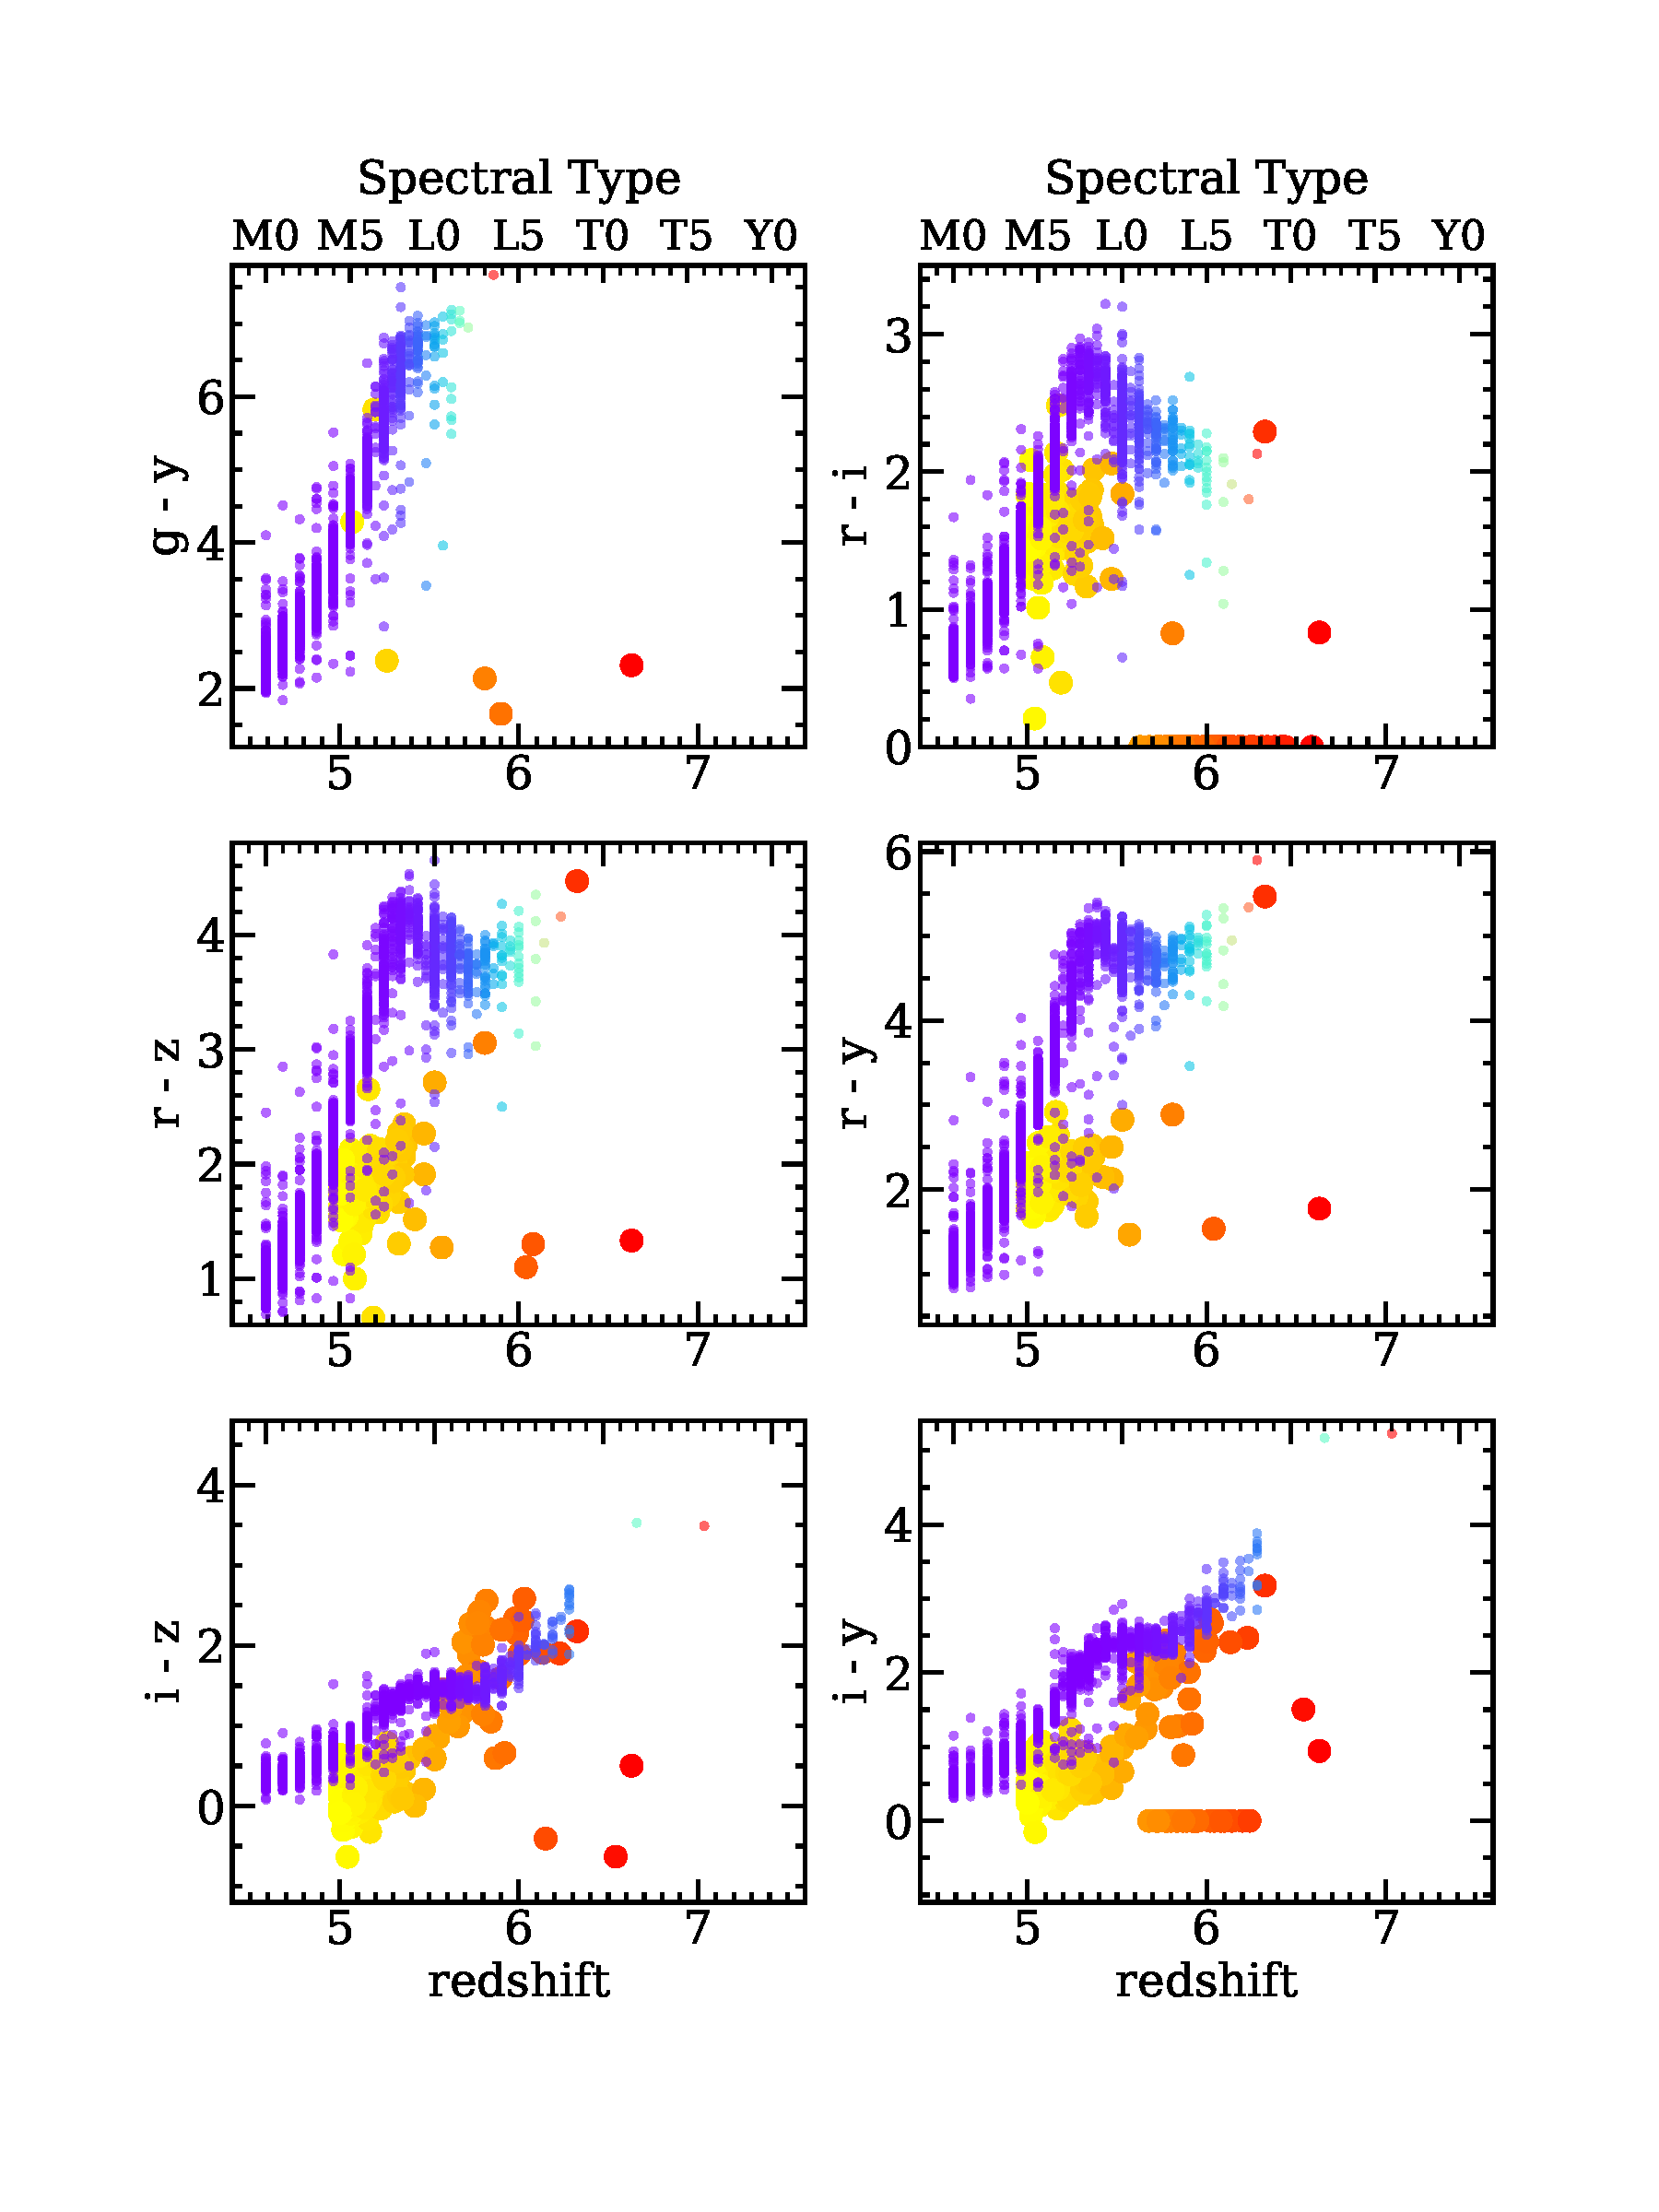
\includegraphics[width=18.0cm]
   {/cos_pc19a_npr/programs/quasars/highest_z/color_redshift/SpecType_vs_Optcolors_20180704.pdf}
   \centering
   \caption[]
   {Optical colour vs. spectral type and redshift for Late Type M/L/T dwarfs and the VH$z$Qs.
     The stars are M, L, and T dwarfs from the \citet{Best2018} PS1-detected catalog.  
   {\it N.B. Trying to look as good as Fig.~5 from Best et al. (2018). How does one get 
bigger gaps between subplots??}}
   \label{fig:Opt_colourredshift}
 \end{figure*}

Figure~\ref{fig:Opt_colourredshift} presents the near-infrared 
colour-redshift trends for Late Type M/L/T dwarfs and the VH$z$Qs.
\begin{figure*}
   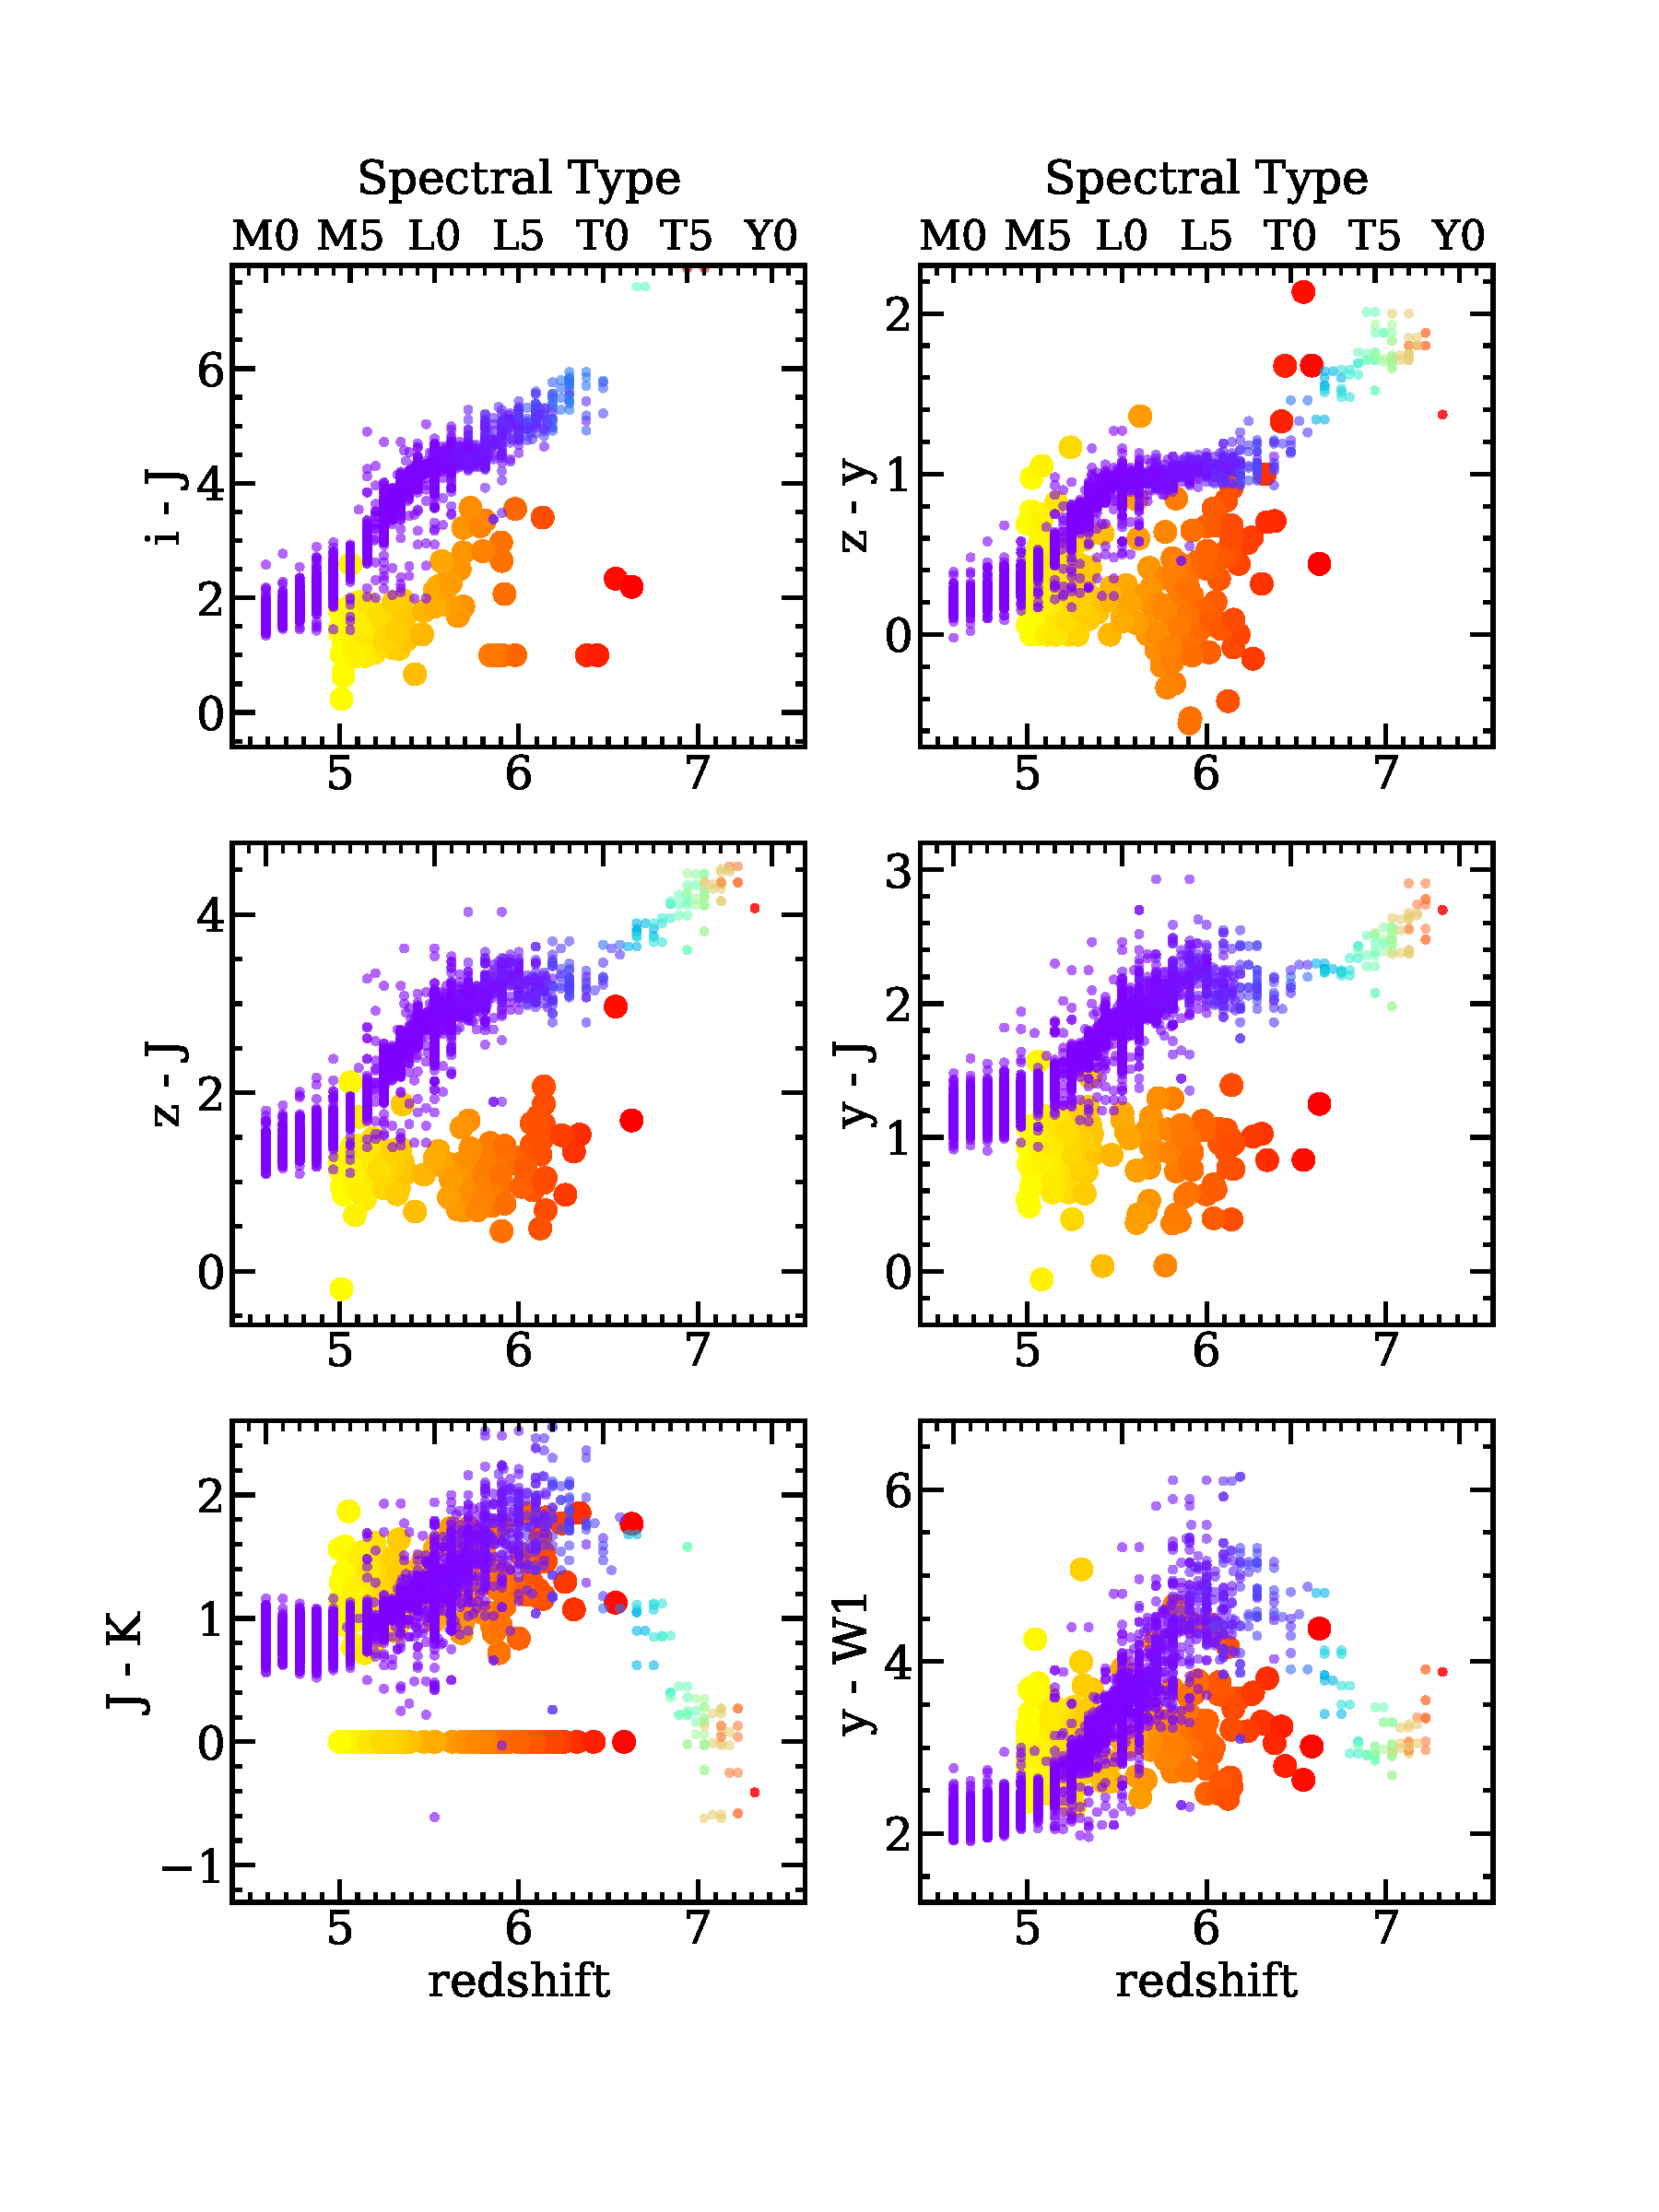
\includegraphics[width=18.0cm]
   {/cos_pc19a_npr/programs/quasars/highest_z/color_redshift/SpecType_vs_NIRcolors_20180704.pdf}
  \centering
   \caption[]
   {Infrared colour-spectral type and redshift plots for Late Type M/L/T dwarfs and the VH$z$Qs.
     {\it NB} I'm really not sure how Best et al. actually get their stellar sequence so clean. 
There are two types of spectral classification,  but restricting it to just SpT\_optn  or SpT\_nir removes
the blue or red end respectively. Hmmm....}
   \label{fig:filters}
 \end{figure*}

\begin{figure*}
   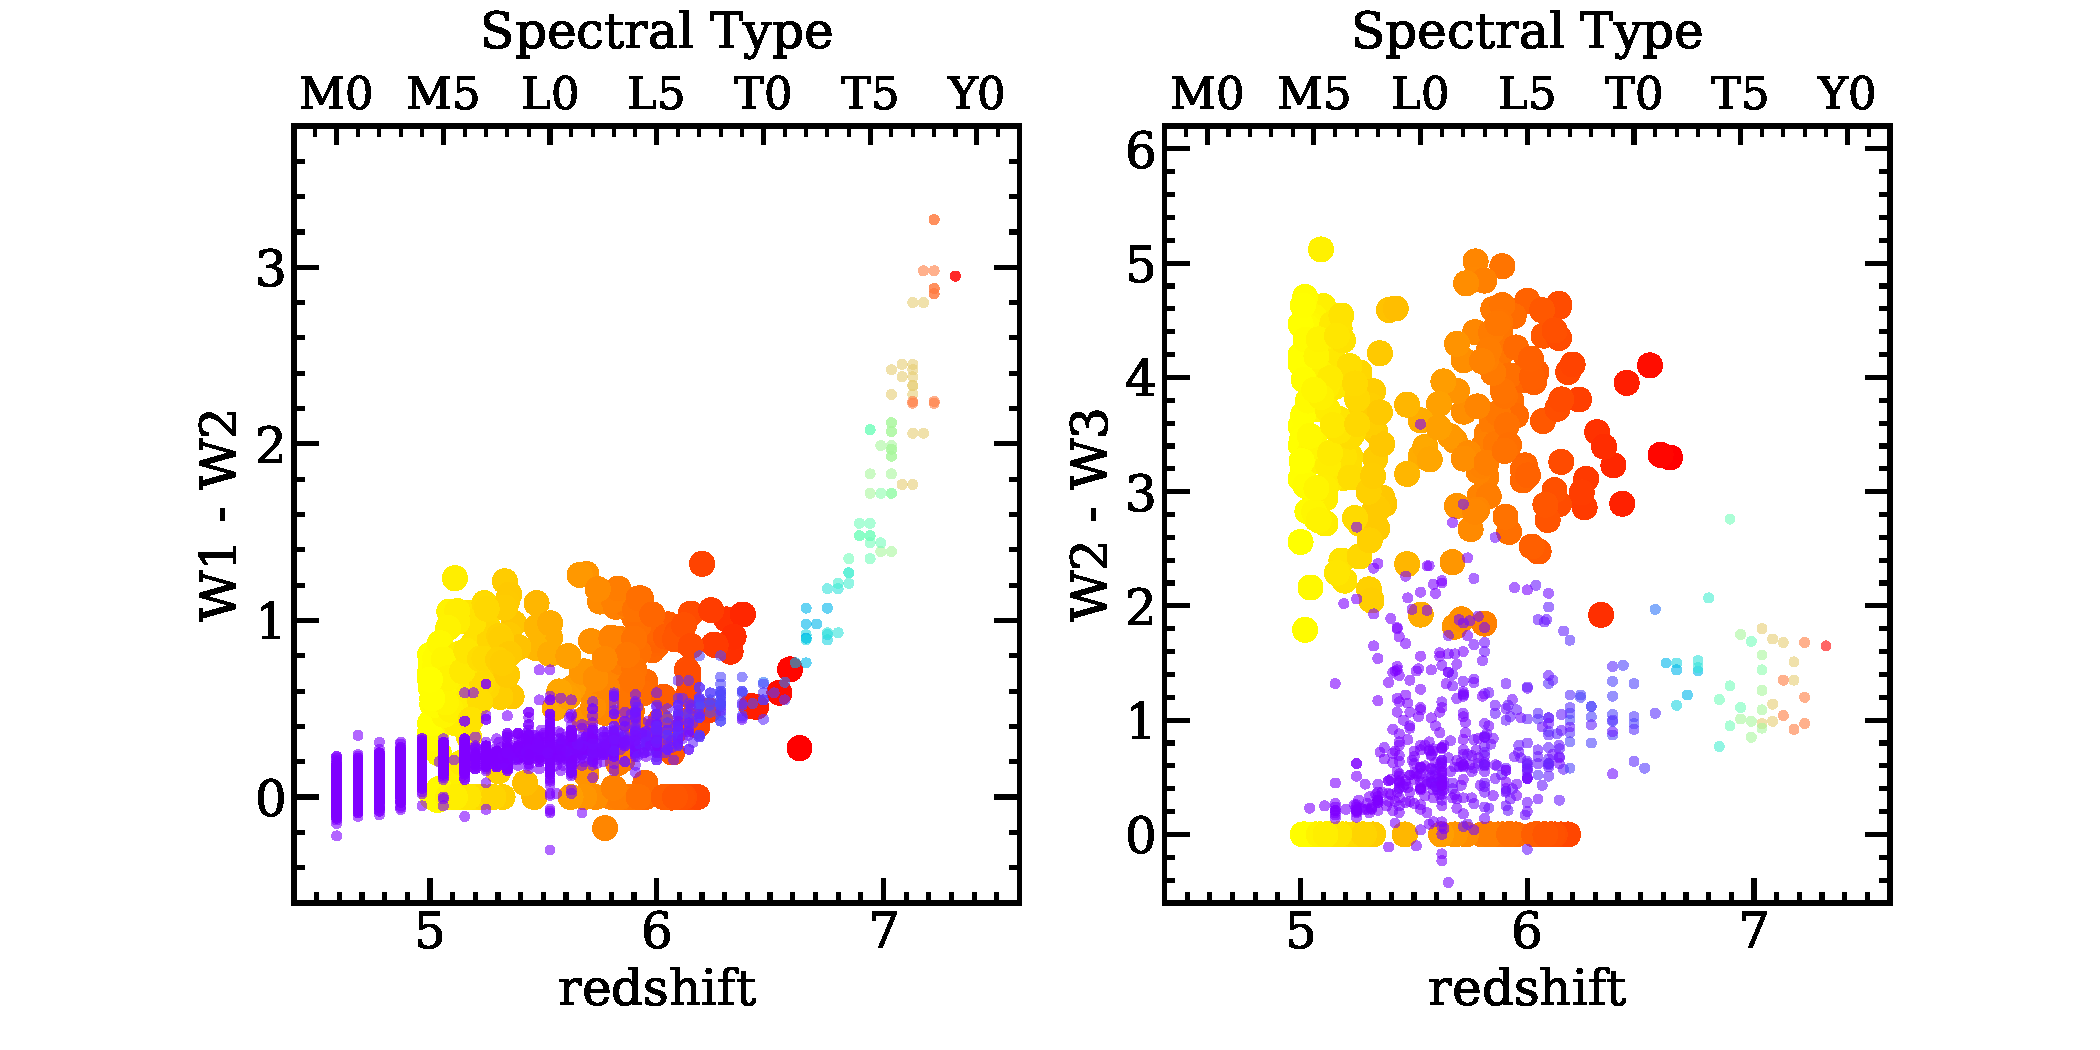
\includegraphics[width=18.0cm]
   {/cos_pc19a_npr/programs/quasars/highest_z/color_redshift/SpecType_vs_W1W2_W2W3colors_20180407.pdf}
  \centering
   \caption[]
   {Infrared colour-spectral type and redshift plots for Late Type M/L/T dwarfs and the VH$z$Qs.
}
   \label{fig:filters}
 \end{figure*}



%\subsection{Number Density of High-$z$ Sources}

\subsection{Consequences of evolution of the $M_{\rm BH} - M_{\star}$ relation}
From a study of 69 {\it Herschel}-detected broad-line active galactic
nuclei, \citet{Sun2015} find there is no evolution in the $M_{\rm BH}
- M_{\star}$ relation from $z\sim2$ to $z\sim0$, with the ratio of
$\log (M_{\rm BH} / M_{\star}$ constant at -2.85 across this redshift
range. If this ratio holds to $z>5$, and we assume the $M_{\rm BH}$
for the $z>6$ measured from the e.g. \mgii line, are generally
correct, then the galaxy total stellar mass for the $z>6$ objects
should be...

\citet{YangG2018} calculate the long-term SMBH accretion rate as a
function of $M_{\rm star}$ and redshift $[BHAR(M_{\star} ,z)]$ over
ranges of $\log (M_{\rm star} / M_{\odot}) = 9.5–12$ and $z = 0.4–4$.
Our BHAR(M⋆,z) is constrained by high-quality survey data
(GOODS-South, GOODS-North and COSMOS), and by the stellar mass
function and the X-ray luminosity function.  This BHAR/SFR dependence
on $M_{\star}$ does not support the scenario that SMBH and galaxy
growth are in lockstep.

\subsection{L-$z$ Plane}
Having obtained an as-near-to-homogenous set of photometry as we can, 
we are now in a position to calculate the Absolute Magnitudes of the VH$z$Q 
sample and in particulare the absolute magnitude at rest-frame 1450\AA'\, $M_{1450}$, 
which is a key physical quantity and goes directly towards the quasar luminosity 
function and thus the reionization of hydrogen calculation. 

At $z=5.00$, the rest-frame 1450\AA\ emission is redshifted to 8700\AA\ iobserved, 
i.e., in the $z$-band, while at 

\begin{figure*}
  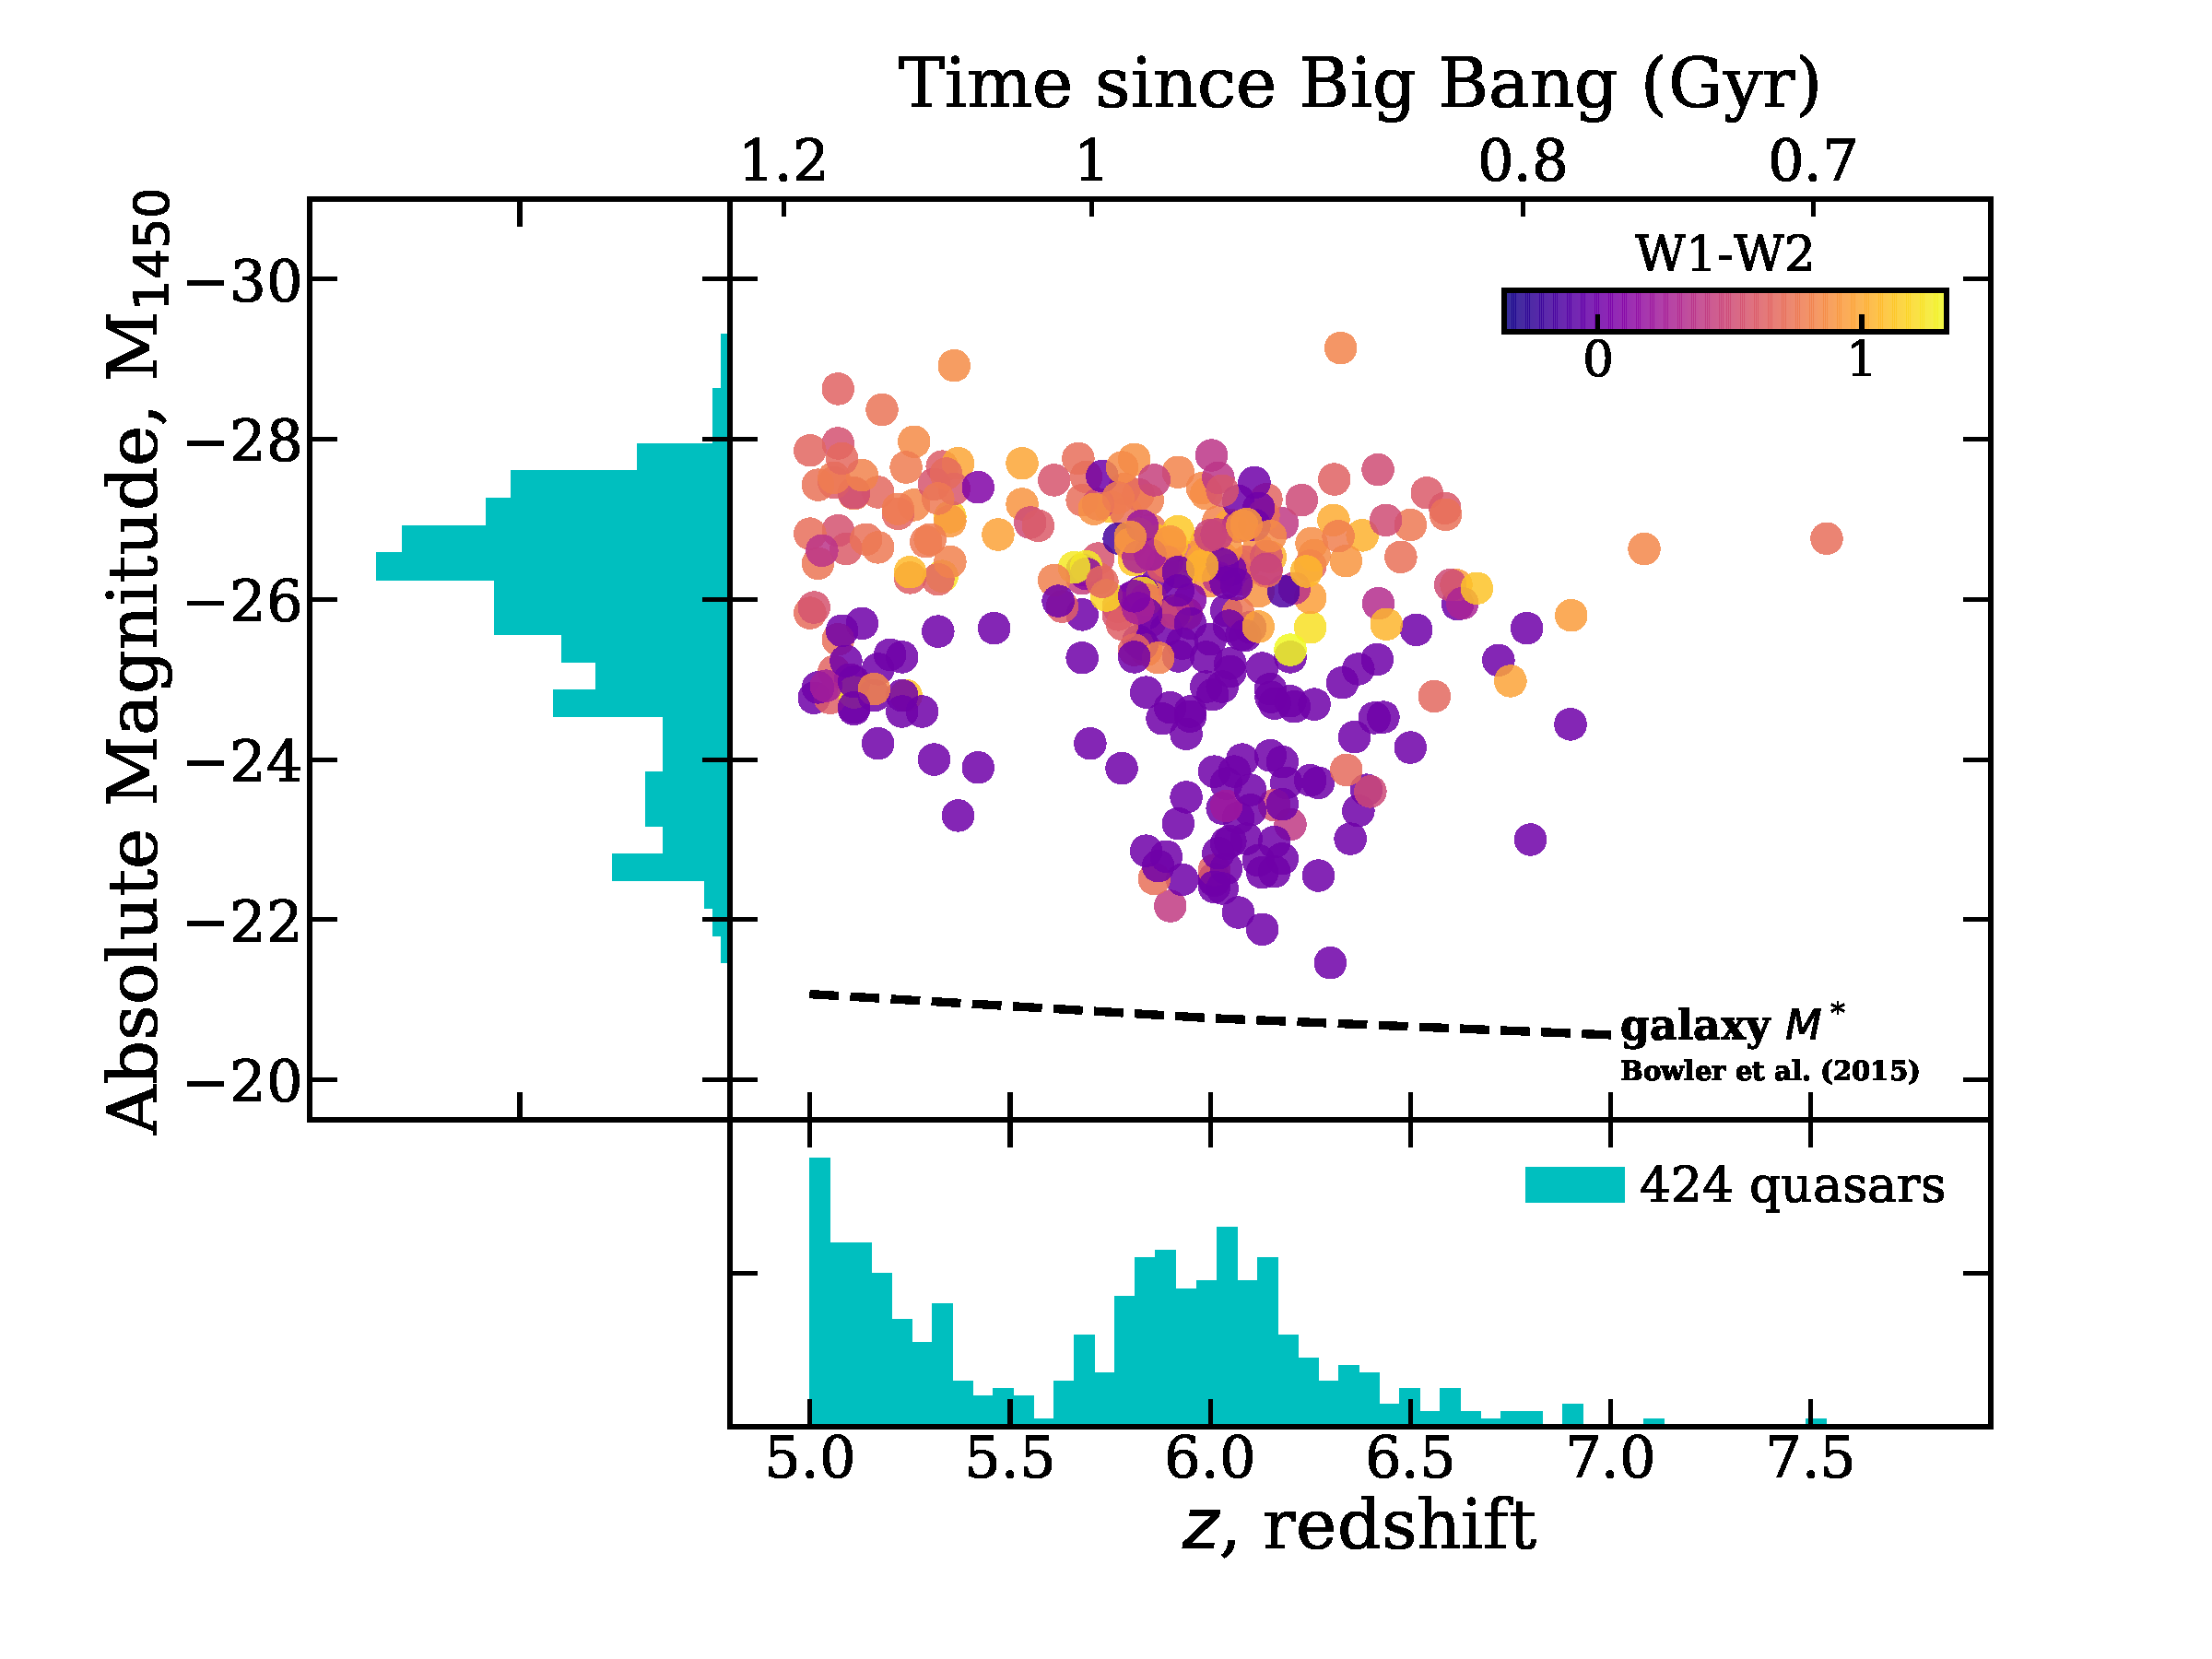
\includegraphics[width=18.0cm]
  {/cos_pc19a_npr/programs/quasars/highest_z/Lz/VHzQ_Lz_20180702.pdf}
  \centering
  \caption[]
  {The spectral bands used by different survey telescopes and that are relevant here.}
  \label{fig:filters}
\end{figure*}


\subsection{SEDs and Dust properties of the VH$z$Qs}
There are a range of IR SEDs e.g. \citet{Mullaney2013} etc. etc. etc. 
However, they are, for our purposes all roughly the same. 

\begin{figure*}
  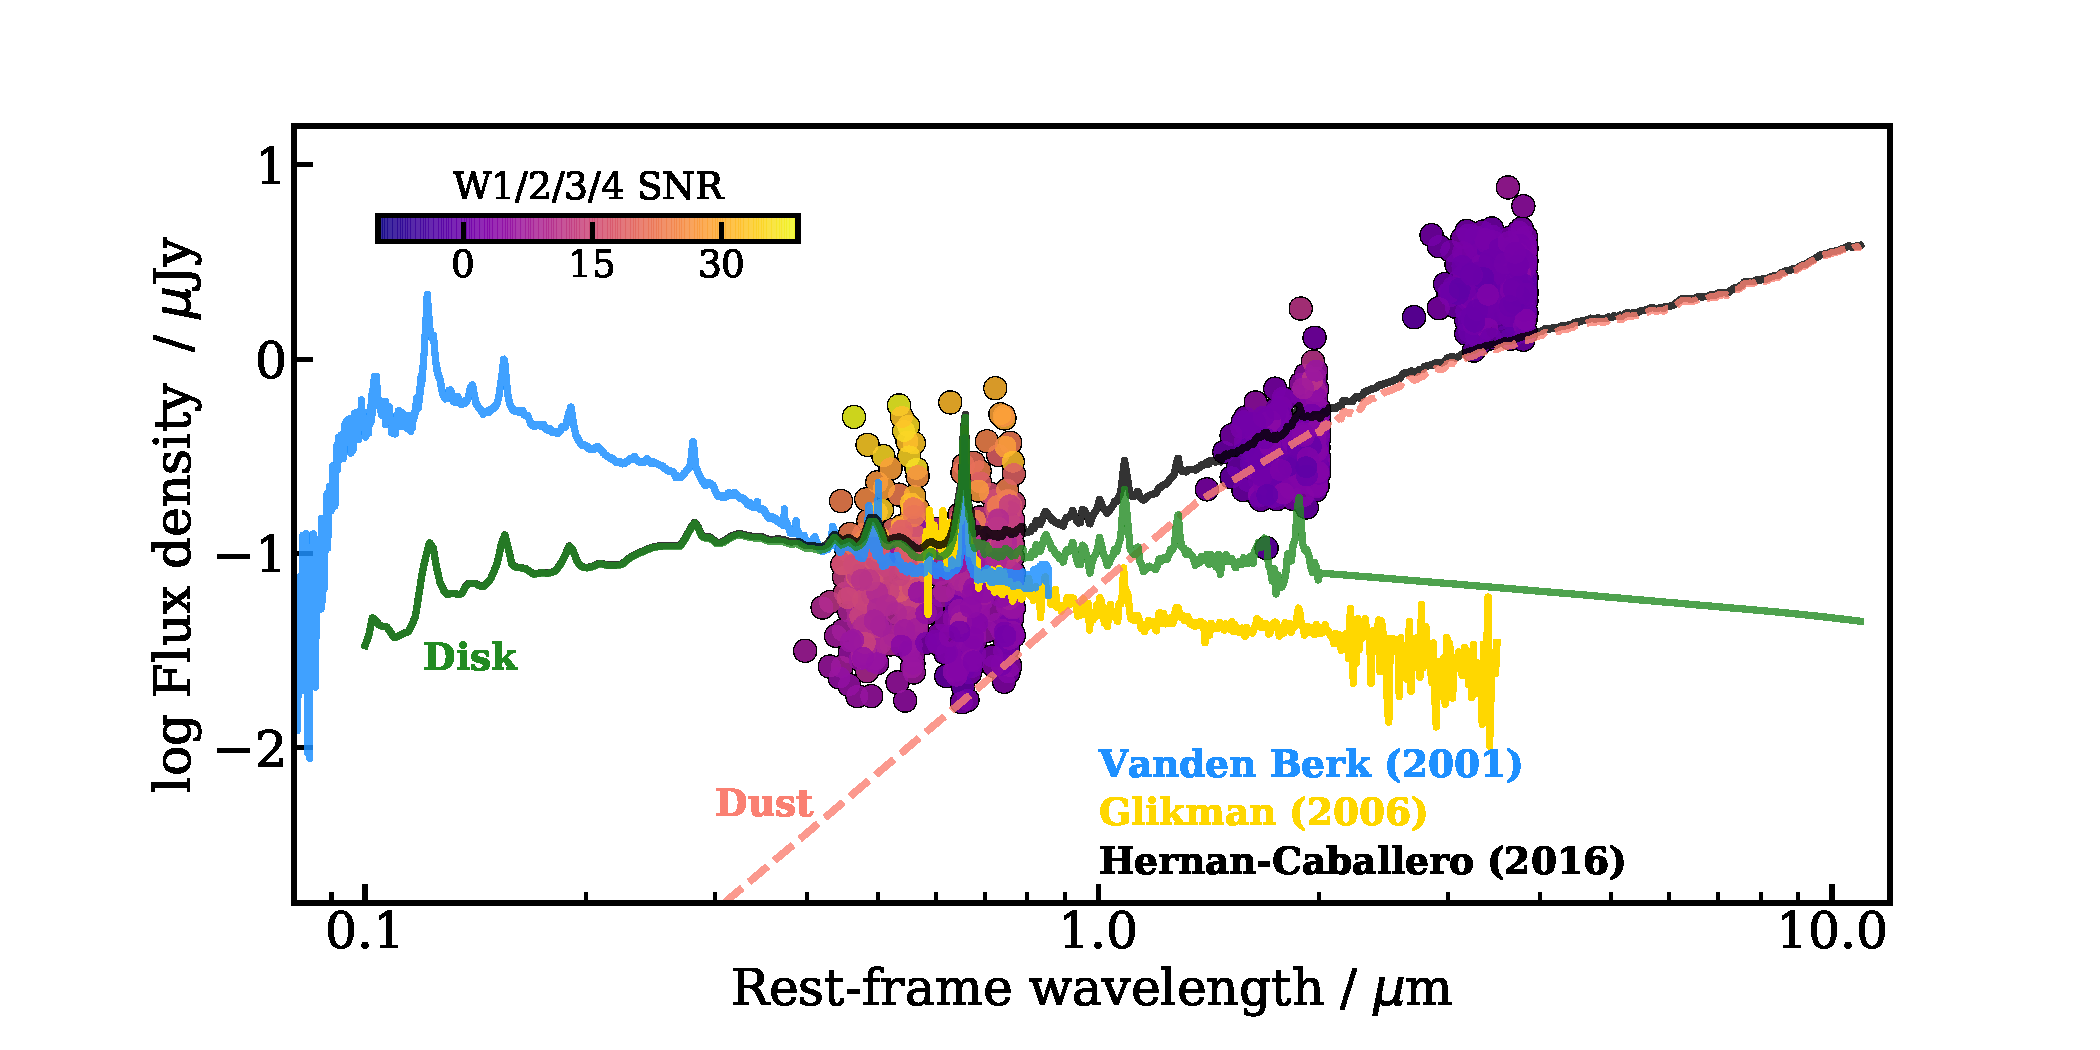
\includegraphics[width=18.0cm]
  {/cos_pc19a_npr/programs/quasars/highest_z/SEDs/RestWavelength_flux_20180702.pdf}
  \centering
  \caption[]
  {The rest-frame properties of the VH$z$Qs. }
  \label{fig:filters}
\end{figure*}



%%%%%%%%%%%%%%%%%%%%%%%%%%%%%%%%%%%%%%%%%%%%%%%%%%%%%%%%%%%%%%%%%%
%%%%%%%%%%%%%%%%%%%%%%%%%%%%%%%%%%%%%%%%%%%%%%%%%%%%%%%%%%%%%%%%%%
%%
%%  S E C T I O  N   7         S E C T I O  N   7           S E C T I O  N   7       S E C T I O  N   7
%%  S E C T I O  N   7         S E C T I O  N   7           S E C T I O  N   7       S E C T I O  N   7
%%  S E C T I O  N   7         S E C T I O  N   7           S E C T I O  N   7       S E C T I O  N   7
%%
%%%%%%%%%%%%%%%%%%%%%%%%%%%%%%%%%%%%%%%%%%%%%%%%%%%%%%%%%%%%%%%%%%
%%%%%%%%%%%%%%%%%%%%%%%%%%%%%%%%%%%%%%%%%%%%%%%%%%%%%%%%%%%%%%%%%%
\section{Discussion and Conclusions}
\label{sec:conclusions}
In this study, we have, for the first time, ompiled the list of all
$z>5$ spectroscopically confirmed quasars. We have assemble the NIR
($y/Y, J, H, K/K_{s}$) and MIR (WISE W1/2/3/4) photometry for these
objects, given their detection rates and SEDs. We find that: 

\begin{itemize}
    \item Lorem ipsum dolor sit amet, consectetur adipiscing
      elit. Aliquam porta sodales est, vel cursus risus porta non. Vivamus
      vel pretium velit. Sed fringilla suscipit felis, nec iaculis lacus
      convallis ac. 
    \item Fusce pellentesque condimentum dolor, quis vehicula
      tortor hendrerit sed. Class aptent taciti sociosqu ad litora torquent
      per conubia nostra, per inceptos himenaeos. Etiam interdum tristique
      diam eu blandit. Donec in lacinia libero.
    \item Sed elit massa, eleifend non sodales a, commodo ut felis. Sed id
      pretium felis. Vestibulum et turpis vitae quam aliquam convallis. Sed
      id ligula eu nulla ultrices tempus. Phasellus mattis erat quis metus
      dignissim malesuada. Nulla tincidunt quam volutpat nibh facilisis
      euismod. Cras vel auctor neque. Nam quis diam risus.
\end{itemize}
Nunc lacus nibh, convallis ac lobortis ut, tempus ac lectus. Maecenas
eu elit massa. Nulla vel lacus lorem. Proin et lobortis
tortor. Phasellus ultrices nisl non enim porttitor dictum. Curabitur
nec nunc ac nibh ornare elementum. Nunc ultrices hendrerit
ultricies. Aliquam dapibus semper est et gravida. Etiam cursus, massa
eget tempor elementum, lectus urna feugiat nisi, eget sagittis.


\section*{Acknowledgements}
NPR acknowledges support from the STFC and the Ernest Rutherford Fellowship scheme. 

We thank Bernie Shiao at STScI for help with the Pan-STARRS1 DR1 CasJobs interface. 

This paper heavily used \href{http://www.star.bris.ac.uk/~mbt/topcat/}{TOPCAT} (v4.4)
\citep[][]{Taylor2005, Taylor2011}.

This research made use of \href{http://www.astropy.org}{\tt Astropy}, 
a community-developed core Python package for Astronomy 
\citep{AstropyCollaboration2013, AstropyCollaboration2018}. 

The Pan-STARRS1 Surveys (PS1) and the PS1 public science archive have
been made possible through contributions by the Institute for
Astronomy, the University of Hawaii, the Pan-STARRS Project Office,
the Max-Planck Society and its participating institutes, the Max
Planck Institute for Astronomy, Heidelberg and the Max Planck
Institute for Extraterrestrial Physics, Garching, The Johns Hopkins
University, Durham University, the University of Edinburgh, the
Queen's University Belfast, the Harvard-Smithsonian Center for
Astrophysics, the Las Cumbres Observatory Global Telescope Network
Incorporated, the National Central University of Taiwan, the Space
Telescope Science Institute, the National Aeronautics and Space
Administration under Grant No. NNX08AR22G issued through the Planetary
Science Division of the NASA Science Mission Directorate, the National
Science Foundation Grant No. AST-1238877, the University of Maryland,
Eotvos Lorand University (ELTE), the Los Alamos National Laboratory,
and the Gordon and Betty Moore Foundation.

CasJobs was originally developed by the Johns Hopkins University/
Sloan Digital Sky Survey (JHU/SDSS) team. With their permission, MAST
used version 3.5.16 to construct CasJobs-based tools for GALEX,
Kepler, the Hubble Source Catalog, and PanSTARRS.

This publication makes use of data products from the Wide-field
Infrared Survey Explorer, which is a joint project of the University
of California, Los Angeles, and the Jet Propulsion
Laboratory/California Institute of Technology, and NEOWISE, which is a
project of the Jet Propulsion Laboratory/California Institute of
Technology. WISE and NEOWISE are funded by the National Aeronautics
and Space Administration.

This research has made use of the SVO Filter Profile Service
(http://svo2.cab.inta-csic.es/theory/fps/) supported from the Spanish
MINECO through grant AyA2014-55216 
%\citet{} 
The SVO Filter Profile Service\footnote{Rodrigo, C., Solano, E., Bayo, A. http://ivoa.net/documents/Notes/SVOFPS/index.html}
describes the Spanish VO Filter Profile Service. 
The Filter Profile Service Access Protocol. Rodrigo, C., Solano, E. http://ivoa.net/documents/Notes/SVOFPSDAL/index.html

\newpage

\appendix
\section{Filter Curves} 
FRom the SVO Filter Profile Service\footnote{http://svo2.cab.inta-csic.es/svo/theory/fps/}.

\section{A. Photometric Bands and Conversions}
    Due to the differing normalizations between the
    SDSS and  UKIDSS photometric systems, certain corrections are required.  To present
    our data in the  purest sense, all the NIR magnitudes from UKIDSS
    (originally AB magnitudes)  were corrected to Vega magnitudes as
    suggested in \citet{Hewett06}.
    
    Although ULAS magnitudes are reported in terms of Vega and SDSS
    magnitudes are reported in AB terms for the most part whenever an
    optical-NIR color was calculated both magnitudes were left in their
    default term.
    
\begin{table*}[h*]
  \begin{center}
   \caption{Adapted from Table 9 of \citet{Peth11}. 
CTIO/DECam, PanSTARRS/PS1, LSST
%References: www.cfht.hawaii.edu/Instruments/Filters/wircam.html
Filter only values. 
}
    \setlength{\tabcolsep}{4pt}
    \begin{tabular}{lcllcl}
      \hline
      \hline
      Band & $\lambda_{\rm eff}  {\buildrel _{\circ} \over {\mathrm{A}}}$ 
              &  $\lambda_{\rm min} {\buildrel _{\circ} \over {\mathrm{A}}}$ 
              & $\lambda_{\rm max} {\buildrel _{\circ} \over {\mathrm{A}}}$ 
              & W$_{\rm eff}$ ${\buildrel _{\circ} \over {\mathrm{A}}}$ 
              & AB - Vega Transformations \\
      \hline
%      {\it u} & 3551  &  3005 &  4000 &  581 & $u$ = $u_{AB}$ - 0.927 \\
%      {\it u_{\rm LSST}} &	3733 &	3182 &	4082 &	?? \\
      $g_{\rm LSST}$      &     4730   &	3877    &	   5665   &  1333   &  $g_{\rm LSST}      = g_{\rm AB} + x $ \\
      $g_{\rm DECam}$  &     4734   & 	3939    &    5528   &   1133   &  $g_{\rm DECam}  = g_{\rm AB} + x $ \\	     
      $g_{\rm PS1}$        &     4776   &    3943    &    5593   &   1167   &  $g_{\rm PS1}      = g_{\rm AB} + x $ \\
      $r_{\rm PS1}$         &     6130  & 	5386    &    7036   &   1318   &  $r_{\rm PS1}       = r_{\rm AB} + y $ \\
      $r_{\rm LSST}$       &     6139  &	5375    &    7055   &   1338   &  $r_{\rm LSST}      = r_{\rm AB} + x $ \\	
      $r_{\rm DECam}$   &     6345  & 	5506    &	   7238   &   1379   &  $r_{\rm DECam}  = r_{\rm AB} + x $ \\	     
      $i_{\rm PS1}$         &     7485  &     6778    &    8304   &   1243   &  $i_{\rm PS1}       = i_{\rm AB} + x $ \\
      $i_{\rm LSST}$       &     7487  &	6765    &	   8325   &   1209   &  $i_{\rm LSST}      = i_{\rm AB} + x $ \\
      $i_{\rm DECam}$   &     7750 &	6950    &    8646    &   1371   &  $i_{\rm DECam}  = i_{\rm AB} + x $ \\	   
      $z_{\rm PS1}$        &     8658 &	8028    &    9346   &      966   &  $z_{\rm PS1}     = z_{\rm AB} + y $ \\
      $z_{\rm LSST}$      &     8669 &	8035    &	   9375   &      994  &   $z_{\rm LSST}      = i_{\rm AB} + x $ \\

      $z_{\rm DECam}$  &     9216 &	8360    &   10166   &   1502  &  $z_{\rm DECam}      = i_{\rm AB} + x $ \\
      $y_{\rm LSST}$      &     9677 &	9089    &	  10859  &     810   &  $y_{\rm LSST}      = i_{\rm AB} + x $ \\
      $Y_{\rm DECam}$   &   10061 &	9400    &   10805   &   1115  &  $Y_{\rm DECam}      = i_{\rm AB} + x $ \\
                                        &            &                   &                 &          &  \\
      $Y_{\rm UKIDSS}$   & 10305 &  9790 & 10810 & 1020 & $Y_{\rm UKIRT}$ = $Y_{AB}$  - 0.634           \\
      $Y_{\rm VISTA}$   & - &  9790 & 10810 & 1020 & $Y_{\rm UKIRT}$ = $Y_{AB}$  - 0.634           \\
      $J_{\rm UKIDSS} $ & 12483 & 11690 & 13280 & 1590 & $J$  = $J_{AB}$- 0.938           \\
      $J_{\rm VISTA} $ & 12483 & 11690 & 13280 & 1590 & $J$  = $J_{AB}$- 0.938           \\
      $W_{\rm Wircam}$ & 14530 &  & & 1020 & $Y$ = $Y_{AB}$  - 0.634           \\
      $H_{\rm UKIDSS}$ & 16313 & 14920 & 17840 & 2920 & $H$ = $H_{AB}$ - 1.379          \\
      $H_{\rm VISTA}$ & 16313 & 14920 & 17840 & 2920 & $H$ = $H_{AB}$ - 1.379          \\
      $K_{\rm UKIDSS}$ & 22010 & 20290 & 23800 & 3510 & $K$ = $K_{AB}$ - 1.9            \\ 
      $K_{\rm VISTA}$ & 22010 & 20290 & 23800 & 3510 & $K$ = $K_{AB}$ - 1.9            \\ 
      \hline
      \hline
      \label{tab:filter_details}
    \end{tabular}
     \end{center}
\end{table*}


\section{PanSTARRS1 SQL queries}\label{sec:PS1_SQL}
The PS1 Casjobs SQL Server is located at
\href{http://mastweb.stsci.edu/ps1casjobs}{mastweb.stsci.edu/ps1casjobs}.
The top level documentation is given
\href{https://outerspace.stsci.edu/display/PANSTARRS/PS1+Source+extraction+and+catalogs}{here}
while the description of tables is given
\href{https://outerspace.stsci.edu/display/PANSTARRS/PS1+Source+extraction+and+catalogs#PS1Sourceextractionandcatalogs}{here}. The
main tables are the
\href{https://outerspace.stsci.edu/display/PANSTARRS/PS1+ObjectThin+table+fields}{{\tt
objectThin}} and
\href{https://outerspace.stsci.edu/display/PANSTARRS/PS1+MeanObject+table+fields}{{\tt
meanObject}} tables.

\section{Near-Infrared WFCAM Science Archive SQL queries}\label{sec:SQL}
Here we give the receipe and SQL that returned the near-infrared photometry 
for the VH$z$Qs. 

\begin{enumerate}
\item http://wsa.roe.ac.uk/ 
\item Login
\item {\tt username:	WSERV1000;  password: 	highzqso;   community: 	nonSurvey} 
\item Freeform SQL Query with  WSERV1000v20180327
\end{enumerate}



\lstset{upquote=true}

\noindent
Then the following SQL will return the values in
Table~\ref{tab:THE_TABLE}.

\begin{lstlisting}[
           language=SQL,
           showspaces=false,
           basicstyle=\ttfamily,
           numbers=left,
           numberstyle=\tiny,
           commentstyle=\color{gray}
        ]
SELECT 
qso.qsoName,  qso.raJ2000 as ra, qso.decJ2000 as dec, 
aver.apertureID,  aver.aperJky3 as aperJky3Aver, 
aver.aperJky3Err as aperJky3AverErr, aver.sumWeight, 
aver.ppErrBits as ppErrBitsAver, m.mjdObs, 
m.filterID, remeas.aperJky3, 
remeas.aperJky3Err, 
w.weight, remeas.ppErrBits, 
m.project

FROM 
finalQsoCatalogue as qso,  
MapApertureIDshighzQsoMap as ma,  
wserv1000MapRemeasAver as aver,  
wserv1000MapRemeasurement as remeas,  
MapProvenance as v,  
wserv1000MapAverageWeights as w, 
MapFrameStatus as mfs, 
Multiframe as m  

WHERE 
qso.qsoID=ma.objectID and 
ma.apertureID=aver.apertureID and 
aver.apertureID=remeas.apertureID and 
aver.catalogueID=v.combicatID and 
v.avSetupID=1 and 
v.catalogueID=remeas.catalogueID and 
w.combicatID=v.combicatID and 
w.catalogueID=v.catalogueID and 
w.apertureID=aver.apertureID and 
mfs.catalogueID=remeas.catalogueID and 
m.multiframeID=mfs.multiframeID and 
mfs.programmeID=10999 and 
mfs.mapID=1 
order by v.combicatID, m.mjdObs
\end{lstlisting}









%%%%%%%%%%%%%%%%%%%%%%%%%%%%%%%%%%%%%%%%%%%%%%%%%%%%%%%%%%%%%%%%%%%%
%%%%%%%%%%%%%%%%%%%%%%%%%%%%%%%%%%%%%%%%%%%%%%%%%%%%%%%%%%%%%%%%%%%%

%\bibliographystyle{apj}
\bibliographystyle{mn2e}
\bibliography{/cos_pc19a_npr/LaTeX/tester_mnras}

\end{document}
